
\documentclass[8pt]{beamer}
\usetheme{default}
\PassOptionsToPackage{usenames,dvipsnames}{xcolor}
\usepackage{my_pres}
\usepackage{tikz}
\usepackage{empheq,accents}
\usepackage{pifont}
\usetikzlibrary{arrows}



% Created by S. Boyd and L. Vandenberghe 
% some traditional definitions that can be blamed on craig barratt
\newcommand{\BEAS}{\begin{eqnarray*}}
\newcommand{\EEAS}{\end{eqnarray*}}
\newcommand{\BEA}{\begin{eqnarray}}
\newcommand{\EEA}{\end{eqnarray}}
\newcommand{\BEQ}{\begin{equation}}
\newcommand{\EEQ}{\end{equation}}
\newcommand{\BIT}{\begin{itemize}}
\newcommand{\EIT}{\end{itemize}}

% text abbrevs
\newcommand{\eg}{{\it e.g.}}
\newcommand{\ie}{{\it i.e.}}

% std math stuff
\newcommand{\ones}{\mathbf 1}
\newcommand{\reals}{{\mbox{\bf R}}}
\newcommand{\integers}{{\mbox{\bf Z}}}
\newcommand{\complex}{{\mbox{\bf C}}}
\newcommand{\symm}{{\mbox{\bf S}}}  % symmetric matrices

% lin alg stuff
\newcommand{\Span}{\mbox{\textrm{span}}}
\newcommand{\range}{{\mathcal R}}
\newcommand{\nullspace}{{\mathcal N}}
\newcommand{\Rank}{\mathop{\bf rank}}
\newcommand{\Tr}{\mathop{\bf tr}}
\newcommand{\cond}{\mathop{\bf cond}}
\newcommand{\diag}{\mathop{\bf diag}}
\newcommand{\lambdamax}{\lambda_{\rm max}}
\newcommand{\lambdamin}{\lambda_{\rm min}}

% probability stuff
\newcommand{\Prob}{\mathop{\bf prob}}
\newcommand{\Expect}{\mathop{\bf E{}}}
\newcommand{\var}{\mathop{\bf var}} % variance
% not sure why we have \Expect and \Prob but \var ???

% convexity & optimization stuff
\newcommand{\Co}{\mathop {\bf conv}} % convex hull
\newcommand{\argmin}{\mathop{\rm argmin}}
\newcommand{\argmax}{\mathop{\rm argmax}}
\newcommand{\epi}{\mathop{\bf epi}}
%\newcommand{\hypo}{\mathop{\bf hypo}}

% sup and inf that look OK in saddle-point form!
%\newcommand{\ourinf}{\mathop{\raisebox{0ex}[0ex][.4ex]{\,inf\,}}}
%\newcommand{\oursup}{\mathop{\raisebox{0ex}[0ex][.4ex]{\,sup\,}}}
\newcommand{\ourinf}{\mathop{\,\mathrm{inf}\, {\rule[-.5ex]{0ex}{0ex}}}}
\newcommand{\oursup}{\mathop{\,\mathrm{sup}\, {\rule[-.5ex]{0ex}{0ex}}}}
%makes latex believe that inf and sup both extend .4ex below
%the baseline

\newcommand{\dist}{\mathop{\bf dist}}
\newcommand{\vol}{\mathop{\bf vol}} % volume
\newcommand{\Card}{\mathop{\bf card}} % cardinality
\newcommand{\sign}{\mathop{\bf sign}}

\newcommand{\dom}{\mathop{\bf dom}} % domain
\newcommand{\aff}{\mathop{\bf aff}} % affine hull
\newcommand{\cl}{\mathop{\bf cl}} % closure
\newcommand{\intr}{\mathop{\bf int}} % interior
\newcommand{\relint}{\mathop{\bf rel int}} % relative interior
\newcommand{\bd}{\mathop{\bf bd}} % boundary

%why do we have the following but not \nust?
\newcommand{\xst}{x^\star}
\newcommand{\lambdast}{\lambda^\star}

% defs for cones & generalized inequalities
% these seem kind of awkward; should fix some day
% rewrite them to use args?
\newcommand{\geqK}{\mathrel{\succeq_K}}
\newcommand{\gK}{\mathrel{\succ_K}}
\newcommand{\leqK}{\mathrel{\preceq_K}}
\newcommand{\lK}{\mathrel{\prec_K}}
\newcommand{\geqKst}{\mathrel{\succeq_{K^*}}}
\newcommand{\gKst}{\mathrel{\succ_{K^*}}}
\newcommand{\leqKst}{\mathrel{\preceq_{K^*}}}
\newcommand{\lKst}{\mathrel{\prec_{K^*}}}
\newcommand{\geqL}{\mathrel{\succeq_L}}
\newcommand{\gL}{\mathrel{\succ_L}}
\newcommand{\leqL}{\mathrel{\preceq_L}}
\newcommand{\lL}{\mathrel{\prec_L}}
\newcommand{\geqLst}{\mathrel{\succeq_{L^*}}}
\newcommand{\gLst}{\mathrel{\succ_{L^*}}}
\newcommand{\leqLst}{\mathrel{\preceq_{L^*}}}
\newcommand{\lLst}{\mathrel{\prec_{L^*}}}

%\newcounter{lecture}
%\newcommand{\lecturefl}[1]{   % use with foiltex landscape
%% \addtocounter{lecture}{1}
% \refstepcounter{lecture}
% \setcounter{equation}{0}
% \setcounter{page}{1}
% \renewcommand{\theequation}{\arabic{equation}}
% \renewcommand{\thepage}{\arabic{lecture}--\arabic{page}}
% \raggedright
% \parindent 0pt
% \rightfooter{\thepage}
% \leftheader{}
% \rightheader{}
% \LogoOff
% \input header 
% \begin{center}
%% {\Large \bfseries Lecture \arabic{lecture} \\*[\bigskipamount] {#1}}
%{\Large \bfseries \arabic{lecture}.  {#1}}
% \end{center}
% \MyLogo{#1}
%}

%\newcommand{\lectureflstar}[1]{   % use with foiltex landscape
% \setcounter{equation}{0}
% \setcounter{page}{1}
% \renewcommand{\theequation}{\arabic{equation}}
% \renewcommand{\thepage}{\arabic{page}}
% \raggedright
% \parindent 0pt
% \rightfooter{\thepage}
% \leftheader{}
% \rightheader{}
% \LogoOff
% \input header 
% \begin{center}
% {\Large \bfseries #1}
% \end{center}
% \MyLogo{#1}
%}
%\newcounter{oursection}
%\newcommand{\frametitle}[1]{  % for use with foiltex landscape
% \addtocounter{oursection}{1}
%% \setcounter{equation}{0}
% \foilhead[-1.0cm]{#1}
% \LogoOn
%}

\newenvironment{algdesc}%
   {\begin{list}{}{%
    \setlength{\rightmargin}{0\linewidth}%
    \setlength{\leftmargin}{.05\linewidth}}%
    \sffamily\small
    \item[]{\setlength{\parskip}{0ex}\hrulefill\par%
    \nopagebreak{}}}%
   {{\setlength{\parskip}{-1ex}\nopagebreak\par\hrulefill} \end{list}}

\newenvironment{colm}{\left[\begin{array}{c}}{\end{array}\right]}
\newenvironment{colv}{\left(\begin{array}{c}}{\end{array}\right)}




\definecolor{texthigh}{RGB}{137, 0, 255}
\definecolor{textred}{RGB}{255, 0, 94}
\definecolor{textgreen}{RGB}{89, 232, 151}
\definecolor{textlightgray}{RGB}{170,170,170}
\definecolor{bggray}{RGB}{230,230,230}
\definecolor{textgray}{RGB}{60,60,60}

\setbeamercolor{background canvas}{bg=bggray}
\setbeamercolor{normal text}{fg=textgray}

\setbeamertemplate{enumerate items}[default]
\setbeamertemplate{itemize items}{\ding{84}}

\title{Informative Data Fusion:\\ Beyond Canonical Correlation Analysis}
\institute[Univ. of Michigan]{\texttt{asendorf@umich.edu}\\[3ex]
Department of Electrical Engineering and Computer
  Science\\University of Michigan\\ }
\author[N. Asendorf]{Nicholas Asendorf}
\date{Dissertation Defense\\[2ex] May 4, 2015}

\newcommand{\twr}{{\sf TW}_\reals}
\newcommand{\twc}{{\sf TW}_\complex}
\newcommand{\sx}{s_{x,i}}
\newcommand{\sy}{s_{y,i}}
\newcommand{\zx}{z_{x,i}}
\newcommand{\zy}{z_{y,i}}
\newcommand{\Zx}{Z_x}
\newcommand{\Zy}{Z_y}
\newcommand{\Ux}{U_x}
\newcommand{\Uy}{U_y}
\newcommand{\Vx}{V_x}
\newcommand{\Vy}{V_y}
\newcommand{\Pxy}{P_{xy}}
\newcommand{\kx}{k_x}
\newcommand{\ky}{k_y}
\newcommand{\kxhat}{\widehat{k}_x}
\newcommand{\kyhat}{\widehat{k}_y}
\newcommand{\khatcca}{\widehat{k}_{\text{cca}}}
\newcommand{\khaticca}{\widehat{k}_{\text{icca}}}
\newcommand{\Uxhat}{\widehat{U}_x}
\newcommand{\Uyhat}{\widehat{U}_y}
\newcommand{\Sigxhat}{\widehat{\Sigma}_x}
\newcommand{\Sigyhat}{\widehat{\Sigma}_y}
\newcommand{\Vxhat}{\widehat{V}_x}
\newcommand{\Vyhat}{\widehat{V}_y}
\newcommand{\Uxtil}{\widetilde{U}_x}
\newcommand{\Uytil}{\widetilde{U}_y}
\newcommand{\Vxtil}{\widetilde{V}_x}
\newcommand{\Vytil}{\widetilde{V}_y}
\newcommand{\Uxcir}{\accentset{\circ}{U}_x}
\newcommand{\Ukcir}{\accentset{\circ}{U}_{\widetilde{K}}}
\newcommand{\Uycir}{\accentset{\circ}{U}_y}
\newcommand{\Sigxcir}{\accentset{\circ}{\Sigma}_x}
\newcommand{\Sigycir}{\accentset{\circ}{\Sigma}_y}
\newcommand{\Vxcir}{\accentset{\circ}{V}_x}
\newcommand{\Vycir}{\accentset{\circ}{V}_y}
\newcommand{\kapcir}{\accentset{\circ}{\kappa}}
\newcommand{\xii}{x_i}
\newcommand{\yii}{y_i}
\newcommand{\Tx}{\Theta_x}
\newcommand{\Ty}{\Theta_y}
\newcommand{\Txhat}{\widehat{\Theta}_x}
\newcommand{\Tyhat}{\widehat{\Theta}_y}
\newcommand{\tx}{\theta^{(x)}}
\newcommand{\ty}{\theta^{(y)}}
\newcommand{\Kxy}{K_{xy}}
\newcommand{\Kxytil}{\widetilde{K}_{xy}}
\newcommand{\Uktil}{U_{\widetilde{K}}}
\newcommand{\Vktil}{V_{\widetilde{K}}}
\newcommand{\Uktilhat}{\widehat{U}_{\widetilde{K}}}
\newcommand{\Vktilhat}{\widehat{V}_{\widetilde{K}}}
\newcommand{\kxy}{k^{xy}}
\newcommand{\defeq}{=:}
\newcommand{\Rxx}{R_{xx}}
\newcommand{\Ryy}{R_{yy}}
\newcommand{\Rxy}{R_{xy}}
\newcommand{\Rxxhat}{\widehat{R}_{xx}}
\newcommand{\Ryyhat}{\widehat{R}_{yy}}
\newcommand{\Rxyhat}{\widehat{R}_{xy}}
\newcommand{\wx}{w_x}
\newcommand{\wy}{w_y}
\newcommand{\wxt}{\widetilde{w}_x}
\newcommand{\wyt}{\widetilde{w}_y}
\newcommand{\wxicca}{\widehat{w}_x^{\text{icca}}}
\newcommand{\wyicca}{\widehat{w}_y^{\text{icca}}}
\newcommand{\wxticca}{\widetilde{w}_x^{\text{icca}}}
\newcommand{\wyticca}{\widetilde{w}_y^{\text{icca}}}
\newcommand{\wxhaticca}{\widehat{w}_x}
\newcommand{\wyhaticca}{\widehat{w}_y}
\newcommand{\Ccca}{C_{\text{cca}}}
\newcommand{\Cccahat}{\widehat{C}_{\text{cca}}}
\newcommand{\Ciccahat}{\widehat{C}_{\text{icca}}}
\newcommand{\Ciccat}{\widetilde{C}_{\text{icca}}}
\newcommand{\rank}{\text{rank}}
\newcommand{\taucca}{\tau_{\text{cca}}^\alpha}
\newcommand{\tauicca}{\tau_{\text{icca}}^\alpha}
\newcommand{\simiid}{\overset{\text{i.i.d.}}{\sim}}
\newcommand{\rhocca}{\rho_\text{cca}}
\newcommand{\rhohatcca}{\widehat{\rho}_\text{cca}}
\newcommand{\rhohaticca}{\widehat{\rho}_\text{icca}}
\newcommand{\rhoeff}{k_{\text{eff}}^{xy}}
\newcommand{\Cmcca}{C_{\text{mcca}}}
\newcommand{\Ucir}{\accentset{\circ}{U}}
\newcommand{\Vcir}{\accentset{\circ}{V}}
\newcommand{\Cmccatil}{\widetilde{C}_{\text{mcca}}}

\newcommand{\iccap}{ICCA\texttt{+} }
\newcommand{\iccaps}{ICCA\texttt{+}}
\newcommand{\Sigxtil}{\widetilde{\Sigma}_x}
\newcommand{\Sigytil}{\widetilde{\Sigma}_y}

\newcommand{\Cmccahat}{\widehat{C}_{\text{mcca}}}
\newcommand{\Cimccahat}{\widehat{C}_{\text{imcca}}}

%\newcommand{\kapcir}{\accentset{\circ}{\kappa}}
%\newcommand{\simiid}{\overset{\text{i.i.d.}}{\sim}}
%\newcommand{\twc}{{\sf TW}_\complex}

%\newcommand{\Uxcir}{\accentset{\circ}{U}_x}
%\newcommand{\Uycir}{\accentset{\circ}{U}_y}
%\newcommand{\Vxcir}{\accentset{\circ}{V}_x}
%\newcommand{\Vycir}{\accentset{\circ}{V}_y}

\begin{document}

%--- the titlepage frame -------------------------%
\begin{frame}[plain]
  \titlepage
  \addtocounter{framenumber}{-1}
\end{frame}

%%%%%%%%%%%%%%%%%%%%%%%%%%%%%%%%%%%%%%%%%%%%%%%%%%%%%%%%%%%%%%%%%%%%%%
\begin{frame}{Motivation}

  \begin{center}
    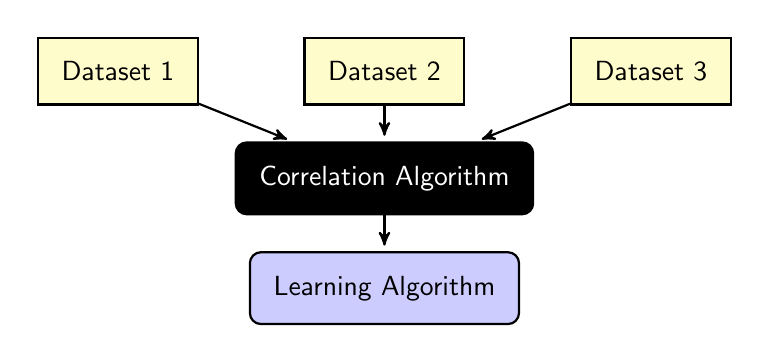
\begin{tikzpicture}[
      font=\sffamily,
      every matrix/.style={ampersand replacement=\&,column sep=3ex,row sep=3ex},
      dataset/.style={draw,thick,fill=yellow!20,inner sep=.3cm},
      sink/.style={dataset,rounded corners,fill=black, text=white},
      app/.style={dataset,rounded corners,fill=blue!20},
      dots/.style={gray,scale=2},
      to/.style={->,>=stealth',shorten >=2pt,thick,font=\sffamily\footnotesize},
      every node/.style={align=center}]

      \matrix{
        \node[dataset] (dataset1) {Dataset 1};
        \& \node[dataset] (dataset2) {Dataset 2};
        \& \node[dataset] (dataset3) {Dataset 3}; \\

        \& \node[sink] (blackbox) {Correlation Algorithm}; \& \\

        \& \node[app] (application) {Learning Algorithm}; \& \\      
      };

      \draw[to] (dataset1) -- (blackbox);
      \draw[to] (dataset2) -- (blackbox);
      \draw[to] (dataset3) -- (blackbox);
      \draw[to] (blackbox) -- (application);

    \end{tikzpicture}
  \end{center}

  \begin{center}
    \textbf{Thesis Goal}\\
    \vspace{1ex}
    \fcolorbox{black}[HTML]{F1F1F1}{\parbox{0.6\textwidth}{%
        \centering Develop theoretically justified, robust\\ correlation algorithms for\\
        multi-dataset fusion}}
  \end{center}

    
\end{frame}

\begin{frame}{A Myriad of Applications}

  \begin{columns}[T]
    \begin{column}{0.45\textwidth}
      
      \vspace{3ex}

      \textbf{Multiple Datasets}
      \begin{itemize}
      \item \textcolor<1>{texthigh}{Audio-Video}
      \item \textcolor<2>{texthigh}{Audio-Audio}
      \end{itemize}

      \hspace{2ex}
      

      \textbf{Machine Learning}
      \begin{itemize}
      \item \textcolor<3>{texthigh}{emotion identification}
      \item \textcolor<4>{texthigh}{shopping predictions}
      \item \textcolor<5>{texthigh}{music genre classification}
      \end{itemize}
      
      \hspace{2ex}

      \textbf{Medical Signal Processing}
      \begin{itemize}
      \item MRI, fMRi, EEG, MEG, etc.
      \end{itemize}


    \end{column}
    \begin{column}{0.45\textwidth}
      \begin{center}
      \includegraphics<1>[width=0.6\textwidth]{figures/parking_lot.jpg}\vspace{3ex}
      \includegraphics<1>[width=0.6\textwidth]{figures/car.png}
      \includegraphics<2>[width=0.8\textwidth]{figures/burton.jpg}
      \includegraphics<3>[width=0.6\textwidth]{figures/emotion1.png}
      \includegraphics<4>[width=0.8\textwidth]{figures/amazon_books.jpg}
      \includegraphics<5>[width=0.8\textwidth]{figures/Queen-Band.jpg}

      \vspace{4ex}

      \includegraphics<1>[width=0.6\textwidth]{figures/parking_lot2.jpg}
      \includegraphics<2>[width=0.8\textwidth]{figures/umich.png}
      \includegraphics<3>[width=0.7\textwidth]{figures/speaker_audio.pdf}
      \includegraphics<4>[width=0.8\textwidth]{figures/amazon_movies.jpg}
      \onslide<5>{\fcolorbox{black}[HTML]{F1F1F1}{\parbox{0.9\textwidth}{%
        \begin{itemize}
        \item disco influences
        \item danceable grooves
        \item repetitive melodic phrasing
        \item extensive vamping
        \item minor key tonality
        \end{itemize}}}}

  \end{center}
    \end{column}
  \end{columns}


\end{frame}


%%%%%%%%%%%%%%%%%%%%%%%%%%%%%%%%%%%%%%%%%%%%%%%%%%%%%%%%%%%%%%%%%%%%%%%%%%%%%%%%%%%%%%%%%%
\begin{frame}{Canonical Correlation Analysis}

  \textbf{What is it?}
  \begin{itemize}
  \item Dimensionality reduction algorithm for exactly 2 datasets, $X,Y$
  \item Correlation coefficients, linear transformations
  \end{itemize}

  \vspace{1ex}

  \textbf{What is it not?}
  \begin{itemize}
  \item Data fusion algorithm
  \end{itemize}
 

  \vspace{1ex}

  \begin{columns}
    \begin{column}{0.35\textwidth}
      \textbf{Covariance matrices}
      \begin{itemize}
      \item $\Rxx = \E{xx^H}$
      \item $\Ryy = \E{yy^H}$
      \item $\Rxy = \E{xy^H}$
      \end{itemize}
    \end{column}
    \begin{column}{0.55\textwidth}
      \begin{center}
        \textbf{Optimization problem}
        \vspace{-1ex}
        \begin{empheq}[box={\mybluebox[5pt][5pt][boxgrey]}]{equation*}
          \begin{aligned}
            & \argmax_{w_x,w_y} &&\rho = w_x^HR_{xy}w_y\\
            & \text{subject to } && w_x^H\Rxx w_x=1\\
            &&&w_y^H\Ryy w_y = 1\\
          \end{aligned}
        \end{empheq}
     \end{center}
    \end{column}
  \end{columns}

  \vspace{1ex}

  \textbf{Variable Transformation}
  \begin{itemize}
  \item $f=\Rxx^{1/2}w_x$
  \item $g=\Ryy^{1/2}w_y$
  \end{itemize}

\end{frame}

%%%%%%%%%%%%%%%%%%%%%%%%%%%%%%%%%%%%%%%%%%%%%%%%%%%%%%%%%%%%%%%%%%%%%%%%%%%%%%%%%%%%%%%%%%
\begin{frame}{Canonical Correlation Analysis}
  \addtocounter{framenumber}{-1}
  \textbf{What is it?}
  \begin{itemize}
  \item Dimensionality reduction algorithm for exactly 2 datasets
  \item Correlation coefficients, linear transformations
  \end{itemize}

  \vspace{1ex}

  \textbf{What is it not?}
  \begin{itemize}
  \item Data fusion algorithm
  \end{itemize}
 

  \vspace{1ex}

  \begin{center}
    \textbf{Optimization problem}
    \vspace{-1ex}
    \begin{empheq}[box={\mybluebox[5pt][5pt][boxgrey]}]{equation*}
      \begin{aligned}
        & \argmax_{f,g} &&\rho = f^H\,\underbrace{R_{xx}^{-1/2}R_{xy}R_{yy}^{-1/2}}_{\Ccca}g\\
        & \text{subject to } && \|f\|_2=1\,,\,\|g\|_2=1\\
      \end{aligned}
    \end{empheq}
  \end{center}


  \vspace{3ex}

  \begin{columns}[t]
    \begin{column}{0.3\textwidth}
      \textbf{Canonical Vectors}
      \begin{itemize}
      \item $w_x = R_{xx}^{-1/2}f$
      \item $w_y = R_{yy}^{-1/2}g$
      \end{itemize}
    \end{column}
    \begin{column}{0.4\textwidth}
      \centering
      \phantom{asdfas}\textbf{Insight}\\[-3ex]
      \begin{empheq}[box={\mybluebox[5pt][5pt][boxgrey]}]{equation*}
        \text{\# correlated signals $=k=\rank(\Ccca)$}
      \end{empheq}

    \end{column}
  \end{columns}

\end{frame}

%%%%%%%%%%%%%%%%%%%%%%%%%%%%%%%%%%%%%%%%%%%%%%%%%%%%%%%%%%%%%%%%%%%%%%%%%%%%%%%%%
\begin{frame}{Empirical CCA}

  \begin{columns}[t]
    \begin{column}{0.5\textwidth}

      \textbf{Training Datasets}
      \begin{itemize}
        \itemsep=1ex
      \item $X=\left[x_1,\dots,x_n\right]$
      \item $Y=\left[y_1,\dots,y_n\right]$
      \end{itemize}
    \end{column}
    \begin{column}{0.5\textwidth}

      \textbf{Sample Covariance Matrices}
      \begin{itemize}
      \item $\Rxxhat=\frac{1}{n}XX^H$
      \item $\Ryyhat=\frac{1}{n}YY^H$
      \item $\Rxyhat=\frac{1}{n}XY^H$
      \end{itemize}
    \end{column}
  \end{columns}

  \vspace{1ex}

  \begin{center}
    \textbf{Estimate}\\
    \fcolorbox{black}[HTML]{F1F1F1}{\parbox{0.4\textwidth}{%
        \be\ba
        &\Cccahat &&= \Rxxhat^{-1/2}\Rxyhat\Ryyhat^{-1/2}\\
        &&&=\widehat{F}\widehat{K}\widehat{G}^H
        \ea\ee
      }}
  \end{center}

      \textbf{Data SVDs}
      \begin{itemize}
        \itemsep=1ex
      \item $X = \Uxhat\Sigxhat\Vxhat^H$
      \item $Y=\Uyhat\Sigyhat\Vyhat^H$
      \item $\sigma\left(\Cccahat\right) = \sigma\left(\Vxhat^H\Vyhat\right)$
      \end{itemize}

\end{frame}

%%%%%%%%%%%%%%%%%%%%%%%%%%%%%%%%%%%%%%%%%%%%%%%%%%%%%%%%%%%%%%%%%%%%%%%%%%%%%%
\begin{frame}{Motivational Example -
    \href{run:/home/asendorf/Documents/thesis_videos/flashing_setup.mp4}{Flashing Light Video}}

  \begin{center}\textbf{Left Camera} \hspace{20ex} \textbf{Right Camera}\\
    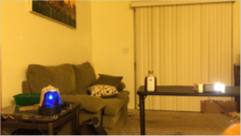
\includegraphics[width=0.47\textwidth]{figures/flashing_left.png}\hspace{2ex}
    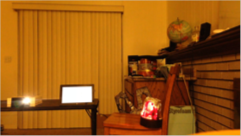
\includegraphics[width=0.47\textwidth]{figures/flashing_right.png}
  \end{center}

  \vspace{2ex}

  \textbf{System parameters}
  \begin{itemize}
  \item Vectorize $135\times 240$ image $\Rightarrow p=q=32400$ pixels
  \item 30 fps @ 30 seconds $\Rightarrow n=900$ frames
  \end{itemize}

  \begin{center}
  \textbf{Goal}\\
  \fcolorbox{black}[HTML]{F1F1F1}{\parbox{0.4\textwidth}{%
      \centering
      Identify correlated pixels between camera views
}}
\end{center}
  

\end{frame}

%%%%%%%%%%%%%%%%%%%%%%%%%%%%%%%%%%%%%%%%%%%%%%%%%%%%%%%%%%%%%%%%%%%%%%%%%%%%%%
\begin{frame}{\href{run:/home/asendorf/Documents/thesis_videos/flashing_cca.mp4}{Empirical
      CCA Results} -
    Canonical Correlations}


    \begin{center}
      \textbf{Top Canonical Correlations }\\
      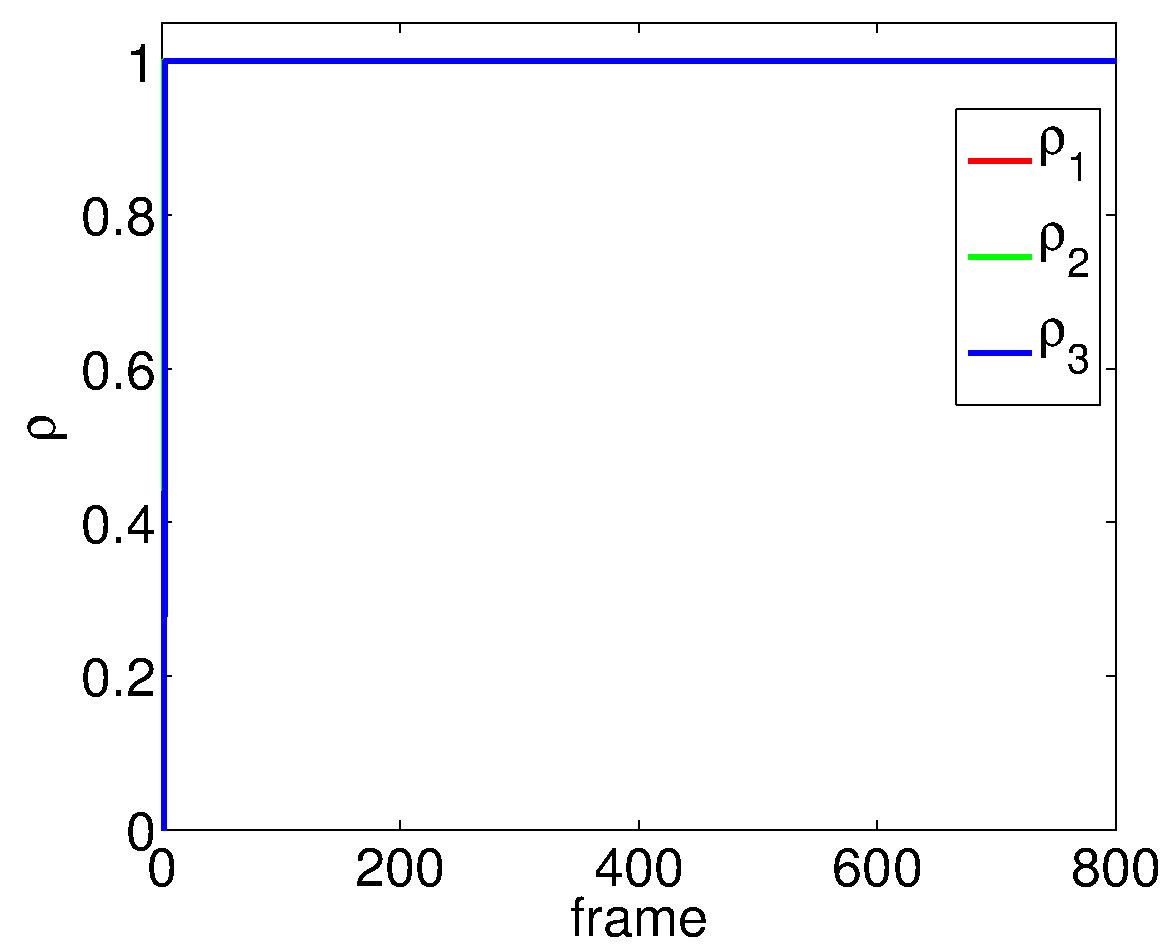
\includegraphics[width=0.5\textwidth]{figures/flashing_cca_corrs.pdf}
    \end{center}


\end{frame}

%%%%%%%%%%%%%%%%%%%%%%%%%%%%%%%%%%%%%%%%%%%%%%%%%%%%%%%%%%%%%%%%%%%%%%%%%%%%%%
\begin{frame}{\href{run:/home/asendorf/Documents/thesis_videos/flashing_cca.mp4}{Empirical
      CCA Results} -
    Canonical Vectors}

  \begin{itemize}
  \item After 900 frames = 30 seconds of video  
  \end{itemize}

  \begin{columns}
    \begin{column}{0.1\textwidth}
      \textbf{Left}\\
      \vspace{15ex}
      \textbf{Right}\\
    \end{column}
    \begin{column}{0.9\textwidth}
      \begin{center}
        \textbf{First} \hspace{15ex} \textbf{Second}\hspace{15ex}\textbf{Third}\\[1ex]
        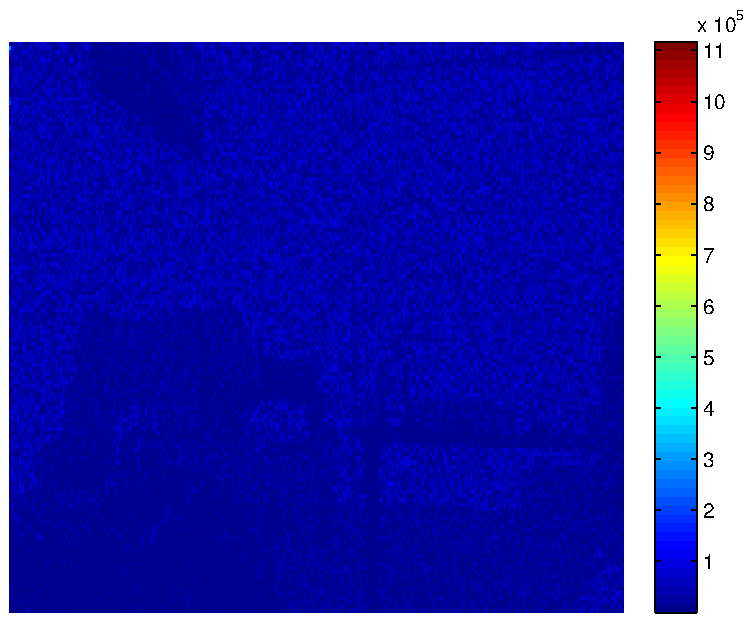
\includegraphics[width=0.3\textwidth]{figures/flashing_cca_wx1.pdf}\hspace{1ex}
        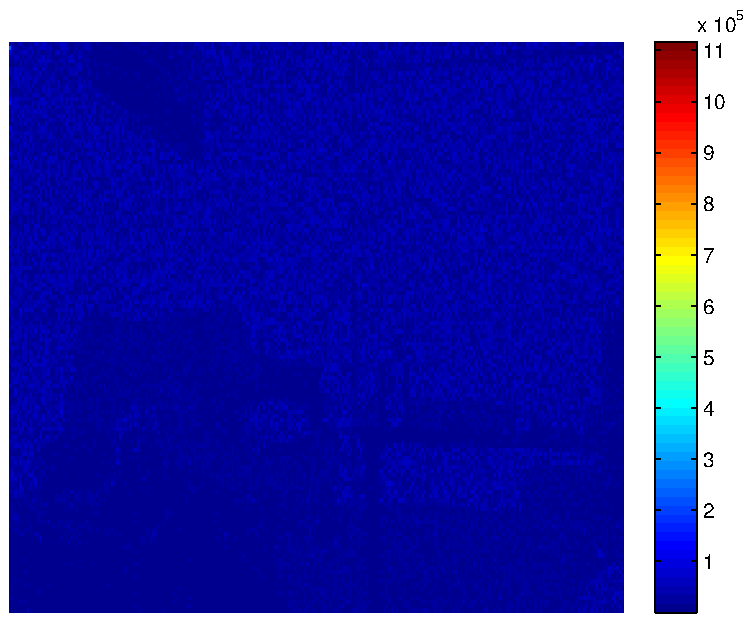
\includegraphics[width=0.3\textwidth]{figures/flashing_cca_wx2.pdf}\hspace{1ex}
        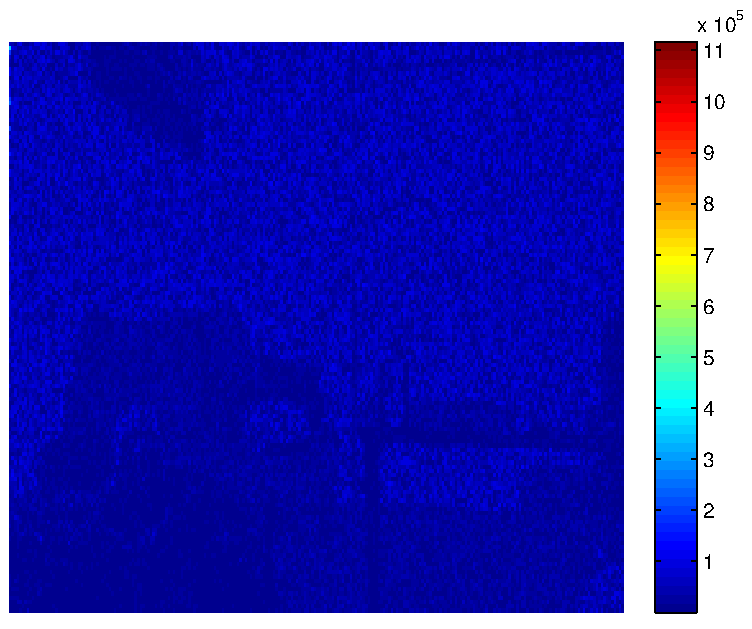
\includegraphics[width=0.3\textwidth]{figures/flashing_cca_wx3.pdf}\\[2ex]
        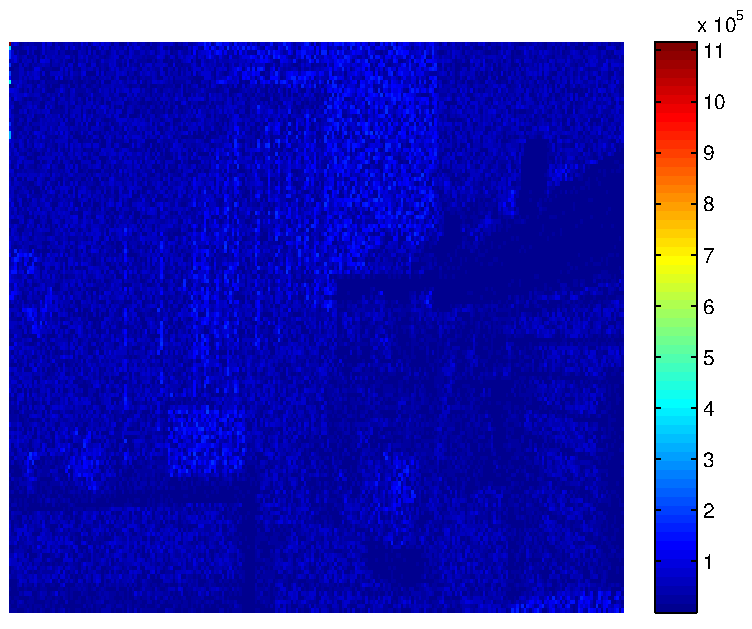
\includegraphics[width=0.3\textwidth]{figures/flashing_cca_wy1.pdf}\hspace{1ex}
        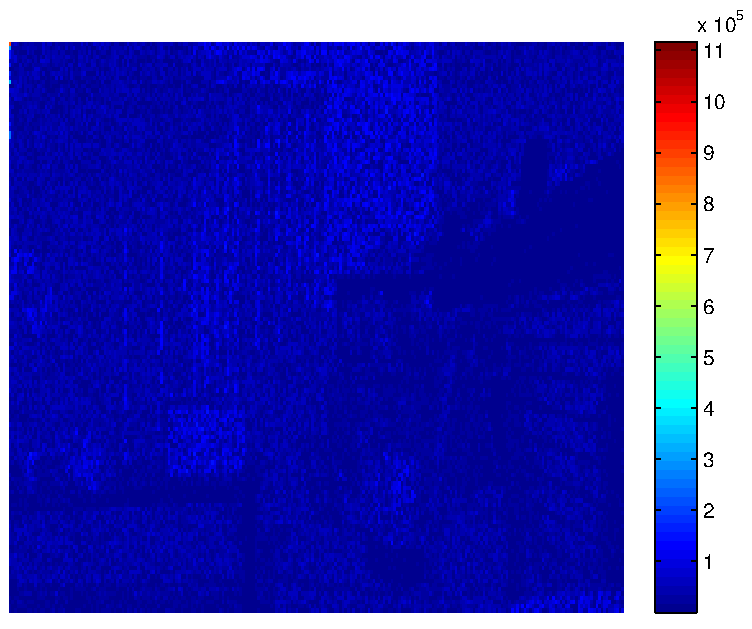
\includegraphics[width=0.3\textwidth]{figures/flashing_cca_wy2.pdf}\hspace{1ex}
        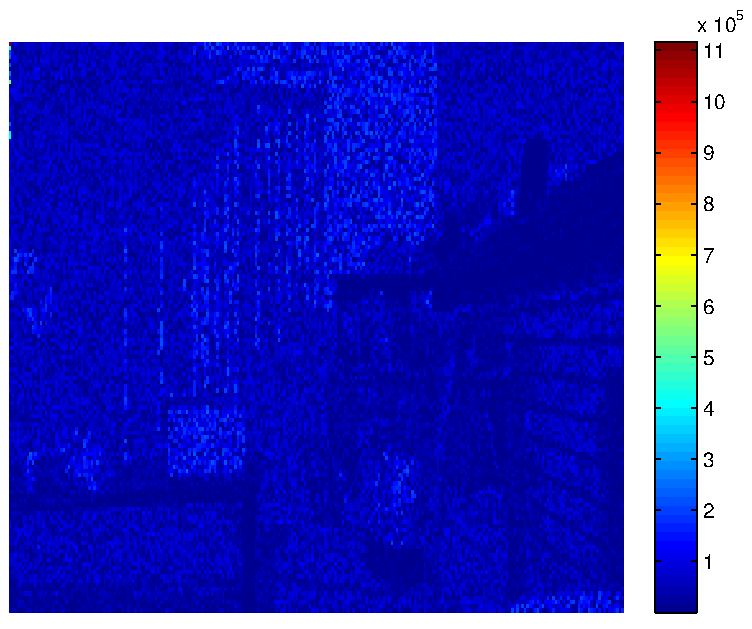
\includegraphics[width=0.3\textwidth]{figures/flashing_cca_wy3.pdf}
      \end{center}
    \end{column}
  \end{columns}

\end{frame}


%%%%%%%%%%%%%%%%%%%%%%%%%%%%%%%%%%%%%%%%%%%%%%%%%%%%%%%%%%%%%%%%%%%%%%%%%%%%%%
\begin{frame}{Previous Observations}

\centering
\fcolorbox{black}[HTML]{F1F1F1}{\parbox{0.8\textwidth}{%
    ``Therefore, the \textcolor{textred}{empirical canonical correlations are defective and
      may not be used} as     estimates of canonical correlations between random
    variables.''
    \begin{flushright}- A. Pezeshki,     L.L. Scharf et al. \\Asilomar Conference on
      Signals Systems and Computer, 2004\end{flushright}

      }}

\vspace{4ex}

\fcolorbox{black}[HTML]{F1F1F1}{\parbox{0.8\textwidth}{%
    ``In conclusion, CCA provide(s) \textcolor{textred}{reliable information} about spatial
    correlations existing among pairs of data sets \textcolor{textred}{only when SNRs ... are
    reasonably high, and the sample support is significantly larger than the data
    dimensions.}''
  \begin{flushright} - H. Ge et al. \\ICASSP, 2009 \end{flushright}}}

\end{frame}

%%%%%%%%%%%%%%%%%%%%%%%%%%%%%%%%%%%%%%%%%%%%%%%%%%%%%%%%%%%%%%%%%%%%%%%%%%%%%%
\begin{frame}{Correlation Analysis Wish List}

  \begin{center}
    \textbf{Correlation Algorithm Wish List}\\[1ex]
\fcolorbox{black}[HTML]{F1F1F1}{\parbox{0.8\textwidth}{%
    \begin{enumerate}
    \item \textbf{Reliable in the sample deficient regime}
      \begin{itemize}
      \item meaningful correlations
      \item meaningful canonical vectors
      \end{itemize}
    \item \textbf{Statistical test for correlations}
      \begin{itemize}
      \item consistency analysis
      \end{itemize}
    \item \textbf{Robust}
      \begin{itemize}
      \item non-gaussian data
      \item missing data
      \end{itemize}
    \item \textbf{Extends to more than 2 datasets}
    \end{enumerate}
}}
\end{center}

\end{frame}

%%%%%%%%%%%%%%%%%%%%%%%%%%%%%%%%%%%%%%%%%%%%%%%%%%%%%%%%%%%%%%%%%%%
\begin{frame}{Thesis Outline}
  \begin{enumerate}
  \item \textcolor{textlightgray}{Introduction}
  \item \textcolor{textlightgray}{Performance of Matched Subspace Detectors Using Finite
      Training Data} 
  \item \textcolor{textlightgray}{Extensions of Deterministic MSD to Missing Data and
      Useful Subspace Components} 
  \item {\color{texthigh}Using CCA and ICCA to Detect Correlations in Low-Rank Signal-Plus-Noise Datasets}
  \item \textcolor{textred}{On Estimating Population Canonical Vectors}
  \item \textcolor{textred}{The Top Singular Values of $XY^H$}
  \item \textcolor{textred}{The Largest Singular Values of a Random Projection of a Low-Rank Perturbation of a Random Matrix} 
  \item \textcolor{textlightgray}{CCA and ICCA for Regression and Detection} 
  \item \textcolor{textred}{Content Based Image Retrieval and Automatic Image Annotation Using Correlations Methods}
  \item \textcolor{textred}{Multiset CCA (MCCA)}
  \end{enumerate}

\end{frame}

%%%%%%%%%%%%%%%%%%%%%%%%%%%%%%%%%%%%%%%%%%%%%%%%%%%%%%%%%%%%%%%%%%%%%%%%%%%%%%%%%%%%%%%%%%
\begin{frame}{Two-Dataset Model}

  \begin{center}
    \textbf{Linear Subspace Model\\}
    \vspace{0.5ex}
    \fcolorbox{black}[HTML]{F1F1F1}{\parbox{0.4\textwidth}{%
        \be\ba
        & x_i = \Ux\sx+\zx\\
        & y_i = \Uy\sy+\zy\\
        \ea\ee
      }}
  \end{center}

  \textbf{Parameters}
  \begin{itemize}
  \item $\Ux^H\Ux = I_{\kx}$, $\Uy^H\Uy = I_{\ky}$
  \item $\zx\simiid\mathcal{CN}(0,I_p)$, \,\,\,$\zy\simiid\mathcal{CN}(0,I_q)$
  \item
    $\E{\left[\begin{array}{c}\sx\\ \sy\end{array}\right]\left[\begin{array}{cc} \sx^H
          & \sy^H \end{array}\right]}= \left[\begin{array}{cc}\Tx & \Kxy\\
        \Kxy^H & \Ty \end{array}\right]$
  \item $\Kxy = \Tx^{1/2}\Pxy\Ty^{1/2}$
  \item $\Theta_x =
    \diag\left(\left(\theta_1^{(x)}\right)^2,\dots,\left(\theta_{k_x}^{(x)}\right)^2\right)$,\,\,\,
    $\Theta_y    =
    \diag\left(\left(\theta_1^{(y)}\right)^2,\dots,\left(\theta_{k_y}^{(y)}\right)^2\right)$  
  \item $\Pxy$ contains correlations $\rho_{kj}$ between signals of $\xii$ and $\yii$
  \item $\widetilde{K}_{xy}
    =\left(\Theta_x+I_{k_x}\right)^{-1/2}K_{xy}\left(\Theta_y+I_{k_y}\right)^{-1/2}$, with
    singular values $\kappa_1,\dots,\kappa_{\min(k_x,k_y)}$
  \end{itemize}
\end{frame}

%%%%%%%%%%%%%%%%%%%%%%%%%%%%%%%%%%%%%%%%%%%%%%%%%%%%%%%%%%%%%%%%%%%%%%%%%%%%%%%%%%%%%%%%%%
\begin{frame}{Statistical Test for Empirical CCA Correlations}

  \textbf{Canonical Correlations}\\[0.25ex]
  \begin{itemize}
  \item $\rhohatcca^{(i)}$ are singular values of $\Cccahat = \Rxxhat^{-1/2}\Rxyhat\Ryyhat^{-1/2}$ 
  \end{itemize}

  \vspace{1ex}

  \begin{center}
    \textbf{Estimate of \# of Correlated Signals }\\[1ex]
    \fcolorbox{black}[HTML]{F1F1F1}{\parbox{0.4\textwidth}{%
        \be
        \widehat{k}_{\text{cca}} = \sum_{i=1}^{\min(p,q)} \indicator_{\left\{\left(\widehat{\rho}_{\text{cca}}^{(i)}\right)^2 >\tau_{\text{cca}}^{\alpha}\right\}}
        \ee
      }}
  \end{center}

  \vspace{3ex}

  \begin{columns}[T]
    \begin{column}{0.6\textwidth}
      \textbf{Setting the threshold}
      \begin{itemize}
      \item $F_{\text{cca}}$ is the cdf of largest singular values of $\Cccahat$ when $X$
        and $Y$ are uncorrelated
      \item $\tau_{\text{cca}}^{\alpha} = F_{\text{cca}}^{-1}(1-\alpha)$ 
      \item $\tau_{\text{cca}}^{\alpha} \approx \sigma_{n,p,q}\twc^{-1}(1-\alpha) + \mu_{n,p,q}$
      \end{itemize}
    \end{column}
    \begin{column}{0.4\textwidth} 
      \centering
      \textbf{Tracy-Widom Distribution}\\
      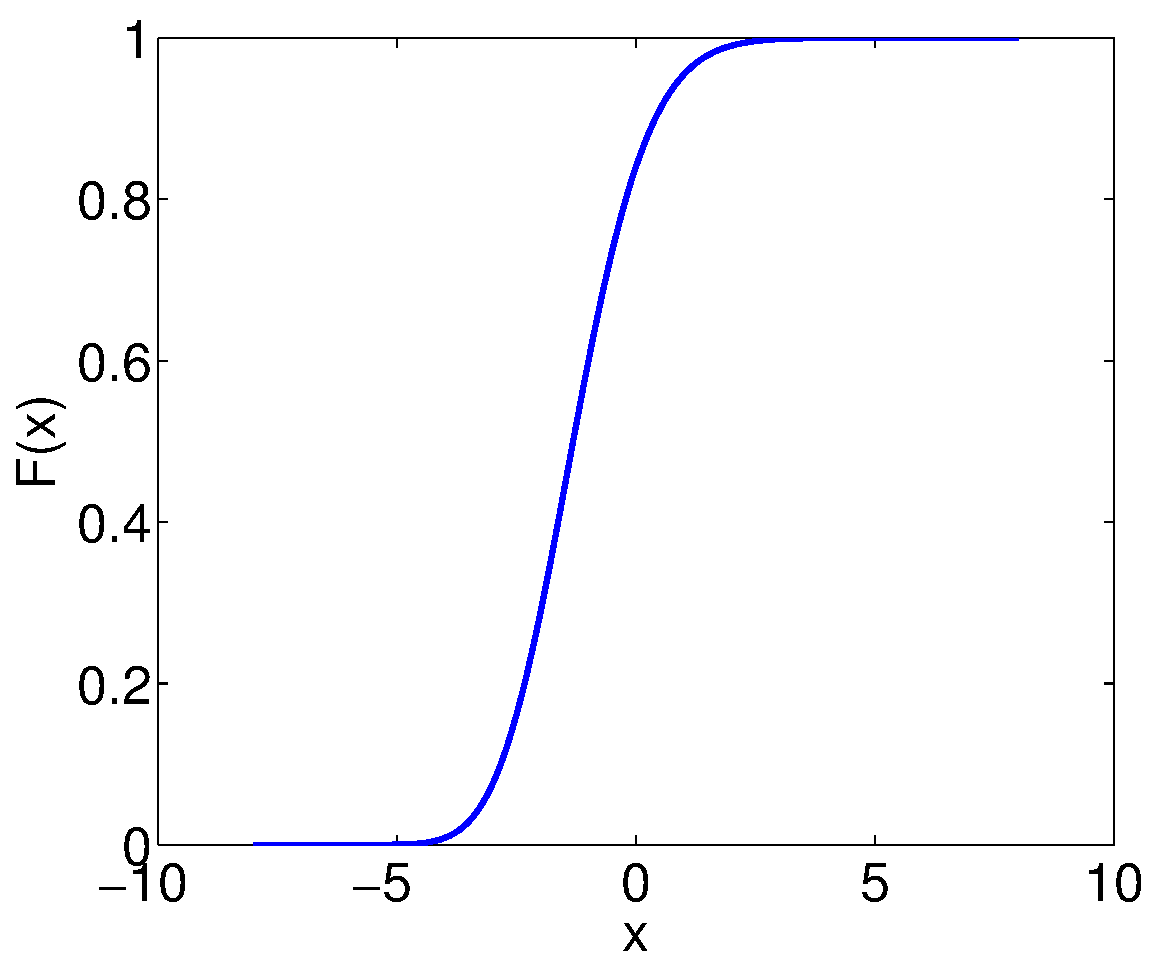
\includegraphics[width=0.95\textwidth]{figures/tw.pdf}
    \end{column}
  \end{columns} 
\end{frame}

%%%%%%%%%%%%%%%%%%%%%%%%%%%%%%%%%%%%%%%%%%%%%%%%%%%%%%%%%%%%%%%%%%%%%%%%%%%%%%%%%%%%%%%%%%
\begin{frame}{Empirical CCA Consistency}

  \begin{prop}[Empirical CCA Consistency, Bao et al.]\label{th:khat_lims}
    Let $p,q,n\to\infty$ with $p/n\to c_x$ and $q/n\to c_y$. Given the above linear subspace
    data model, 
    \be\ba
    & \widehat{k}_{\text{cca}} \convas k &&\text{ if } n>p+q \text{ and } \kappa_k^2 >r_c \\
    \ea\ee
    where
    \be
    r_c = \frac{c_xc_y+\sqrt{c_yc_y(1-c_x)(1-c_y)}}{(1-c_x)(1-c_y) + \sqrt{c_xc_y(1-c_x)(1-c_y)}}.
    \ee
  \end{prop}

  \vspace{3ex}

  \textbf{Recall}
  \begin{itemize}
  \item $\widetilde{K}_{xy}
    =\left(\Theta_x+I_{k_x}\right)^{-1/2}\Tx\Pxy\Ty\left(\Theta_y+I_{k_y}\right)^{-1/2}$
  \item Singular values $\kappa_1,\dots,\kappa_{\min(k_x,k_y)}$
  \end{itemize}

\end{frame}

%%%%%%%%%%%%%%%%%%%%%%%%%%%%%%%%%%%%%%%%%%%%%%%%%%%%%%%%%%%%%%%%%%%%%%%%%%%%%%%%
\begin{frame}{Empirical CCA Consistency}

  \textbf{Simulation parameters}
  \begin{itemize}
  \item $p=q=150$, $k=1$, $\theta=\theta_x=\theta_y$, $\alpha=0.01$
  \end{itemize}

  \vspace{1ex}

  \begin{center}  $\boldsymbol{\rho=}\mathbf{0.7}$\hspace{25ex}$\boldsymbol{\rho=0.9}$\\[0.5ex]
  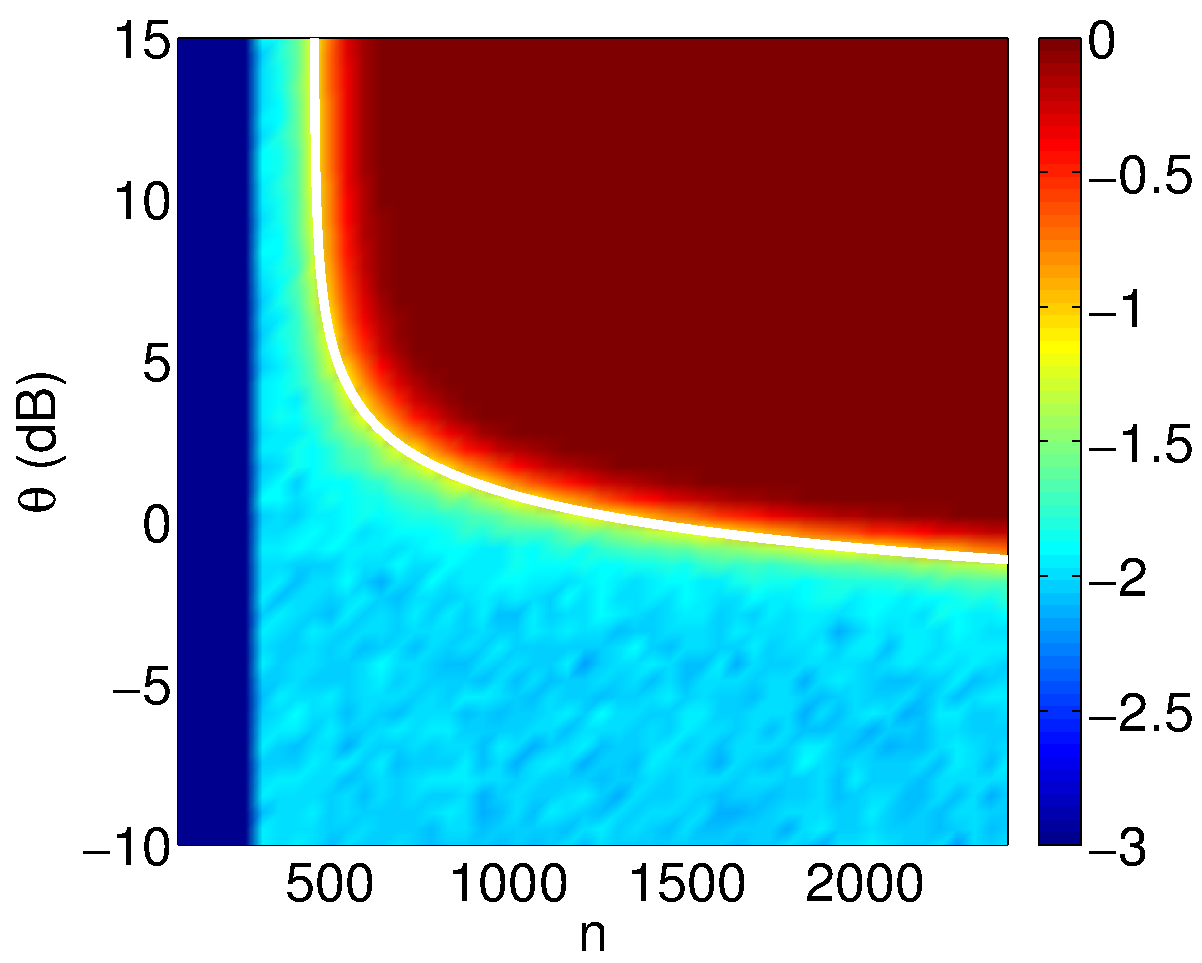
\includegraphics[width=0.4\textwidth]{figures/cca_rho_noicca_7.pdf}\hspace{2ex}
  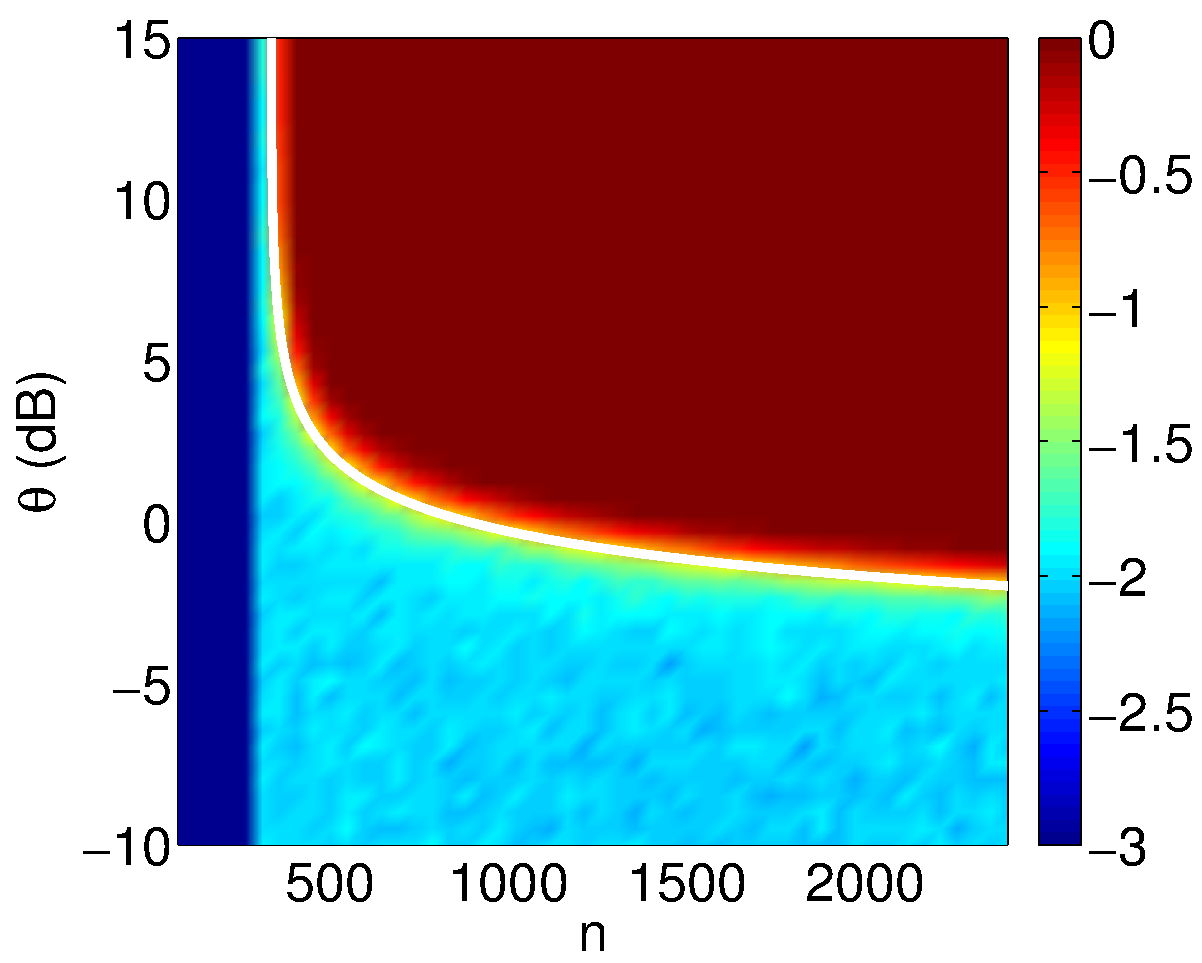
\includegraphics[width=0.4\textwidth]{figures/cca_rho_noicca_9.pdf}
\end{center}



  
  \textbf{Problems!}
  \begin{itemize}
  \item Degenerate case: $\rho=1$ when $n<p+q$ (Pezeshki 2004)
  \item Consistency boundary is dependent on correlation
  \end{itemize}

\end{frame}

%%%%%%%%%%%%%%%%%%%%%%%%%%%%%%%%%%%%%%%%%%%%
\begin{frame}{Informative CCA (ICCA)}


  \textbf{Not all singular vectors are informative!} (Nadakuditi, 2011)
  \begin{itemize}
  \item $\sigma_i\left(\Cccahat\right) = \sigma_i\left(\Vxhat^H\Vyhat\right)$
  \item Trim data SVD's to only use informative components
  \end{itemize}

  \vspace{2ex}

  \fcolorbox{black}[HTML]{F1F1F1}{\parbox{0.9\textwidth}{%
  \begin{enumerate}
    \itemsep=1ex
  \item Trim data SVD's: $X=\widehat{U}_x\,\widehat{\Sigma}_x\,\widehat{V}_x^H$ and $Y=\widehat{U}_y\,\widehat{\Sigma}_y\, \widehat{V}_y^H$
    \begin{itemize}
    \item $\Uxcir = \widehat{U}_x\left(:\,,1:\widehat{k}_x\right)$, $\Uycir = \widehat{U}_y\left(:\,,1:\widehat{k}_y\right)$
    \item $\Vxcir = \widehat{V}_x\left(:\,,1:\widehat{k}_x\right)$, $\Vycir = \widehat{V}_y\left(:\,,1:\widehat{k}_y\right)$
    \end{itemize}

  \item Form
    $\Ciccahat=\Uxcir\Vxcir^H\Vycir\Uycir$
  \item Take SVD: $\Ciccahat = \widetilde{F}\widetilde{K}\widetilde{G}^H$
  \item $\widehat{\rho}_{\text{icca}}^{(i)} = \widetilde{k}_i$
  \item $\widetilde{w}_x^{(i)}=\widehat{R}_{xx}^{-1/2}\,\widetilde{f}_i$
  \item $\widetilde{w}_y^{(i)}=\widehat{R}_{yy}^{-1/2}\,\widetilde{g}_i$
  \end{enumerate}}}

\end{frame}

%%%%%%%%%%%%%%%%%%%%%%%%%%%%%%%%%%%%%%%%%%%%%%%%%%%%%%%%%%%%%%%%%%%%%%%%%%%%%%%%
\begin{frame}{Statistical Test for ICCA Correlations}


  \begin{center}
    \textbf{Estimate of \# of Correlated Signals }\\[1ex]
    \fcolorbox{black}[HTML]{F1F1F1}{\parbox{0.4\textwidth}{%
        \be
        \widehat{k}_{\text{icca}} = \sum_{i=1}^{\min(\widehat{k}_x,\widehat{k}_y)} \indicator_{\left\{\left(\widehat{\rho}_{\text{icca}}^{(i)}\right)^2 >\tau_{\text{icca}}^{\alpha}\right\}}
        \ee
      }}
  \end{center}

  \textbf{Setting the threshold}
  \begin{itemize}
  \item $F_{\text{icca}}$ is the cdf of largest singular values of $\Ciccahat$ in the null setting
    of no correlation
  \item $\tau_{\text{icca}}^{\alpha} = F_{\text{icca}}^{-1}(1-\alpha)$ 
  \item $\tau_{\text{icca}}^{\alpha} \approx \sigma_{n,\kxhat,\kyhat}\twc^{-1}(1-\alpha) + \mu_{n,\kxhat,\kyhat}$
  \end{itemize}


  \begin{Th}[ICCA Consistency]\label{th:khat_lims}
    Let $p,q,n\to\infty$ with $p/n\to c_x$ and $q/n\to c_y$. Given the linear subspace
    data model, 
    \be\ba
    & \widehat{k}_{\text{icca}} \convas k && \text{ if } \min_{i=1,\dots,k_x} \theta_i^{(x)}>c_x^{1/4} \text{ and }
    \min_{i=1,\dots,k_y} \theta_i^{(y)}>c_y^{1/4} 
    \ea\ee
  \end{Th}
\end{frame}

%%%%%%%%%%%%%%%%%%%%%%%%%%%%%%%%%%%%%%%%%%%%%%%%%%%%%%%%%%%%%%%%%%%%%%%%%%%%%%%%
\begin{frame}{Empirical CCA and ICCA Consistency}
  \begin{itemize}
  \item $p=q=150$, $k=1$, $\theta = \theta_x=\theta_y$,$\alpha=0.01$
  \end{itemize}

  \begin{columns}[T]
  \begin{column}{0.01\textwidth}
    \vspace{15ex}
    \textbf{ CCA}\\
    \vspace{20ex}
    \textbf{ICCA}
  \end{column}
  \begin{column}{1\textwidth}
    \begin{center}
      $\boldsymbol{\rho=}\mathbf{0.7}$\hspace{23ex}$\boldsymbol{\rho=0.9}$\\[0.5ex]

        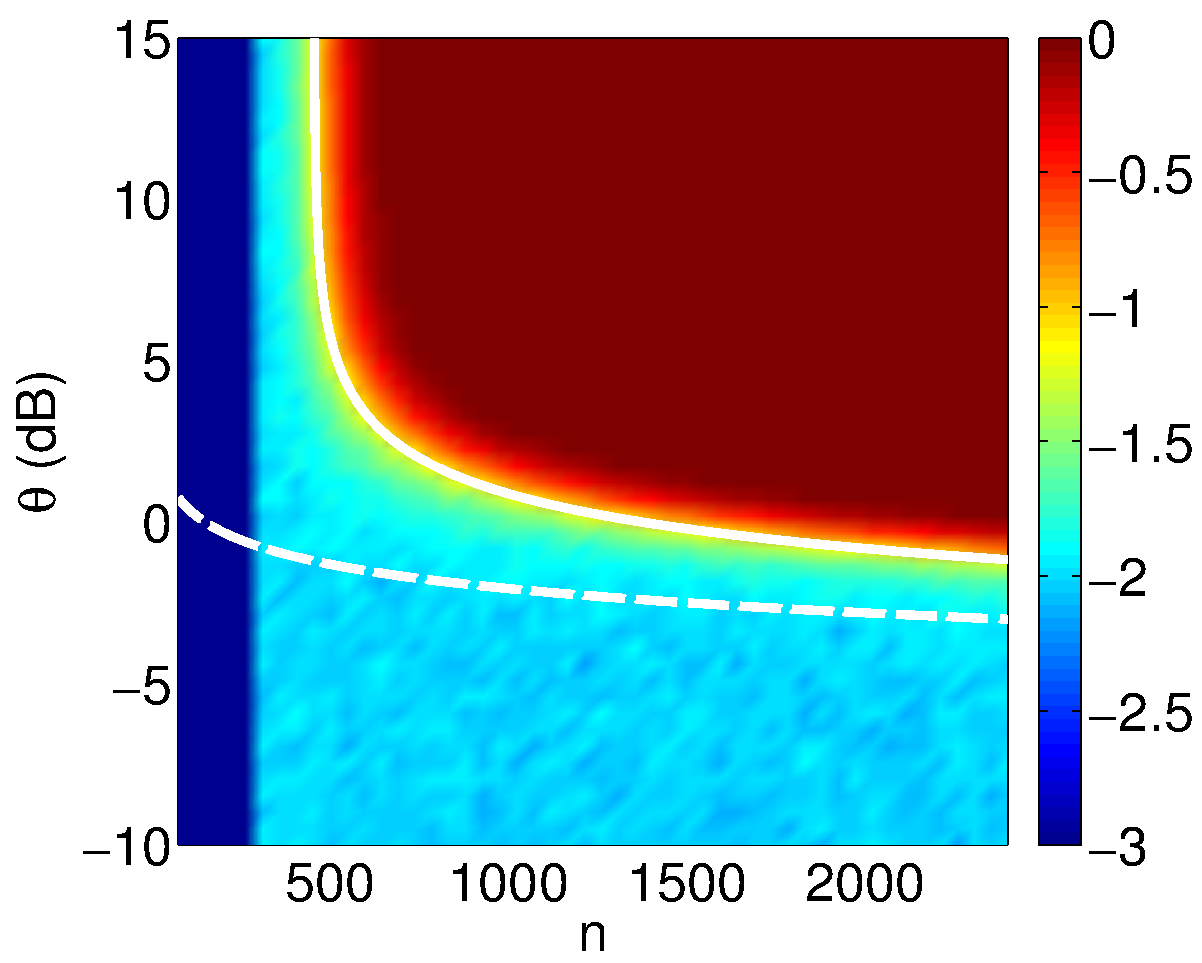
\includegraphics[width=0.35\textwidth]{figures/cca_rho7.pdf}\hspace{2ex}
        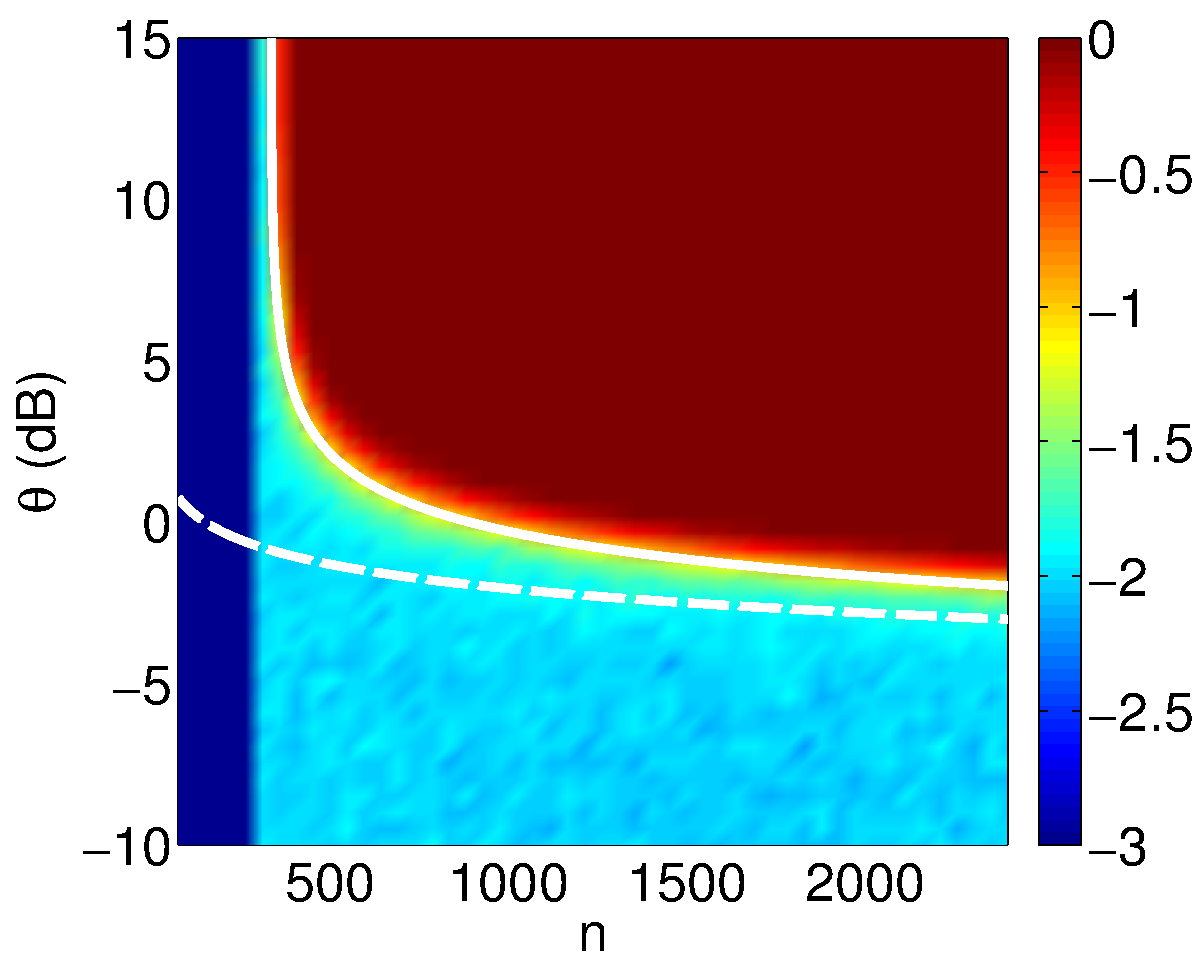
\includegraphics[width=0.35\textwidth]{figures/cca_rho9.pdf}\\[2ex]
        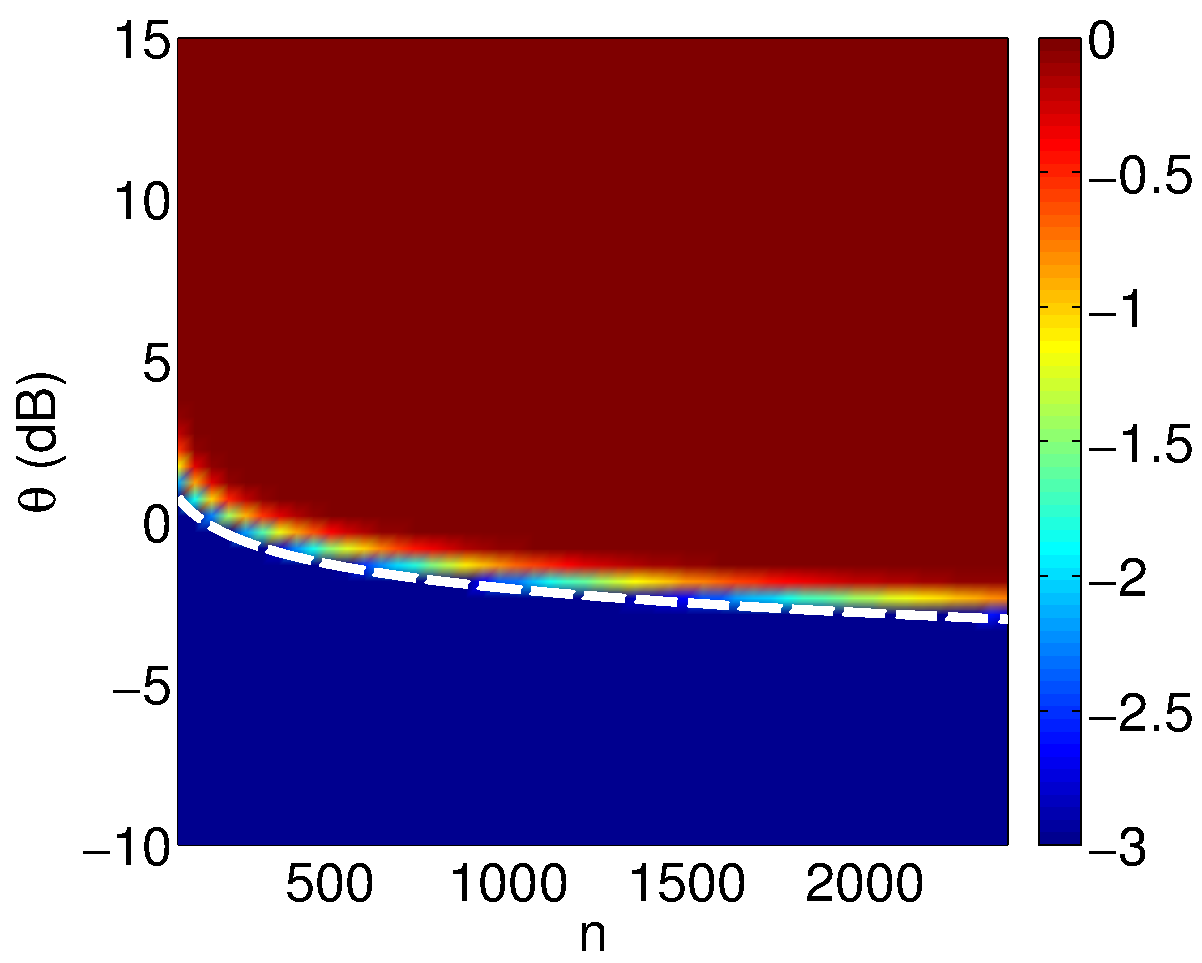
\includegraphics[width=0.35\textwidth]{figures/icca_rho7.pdf}\hspace{2ex}
        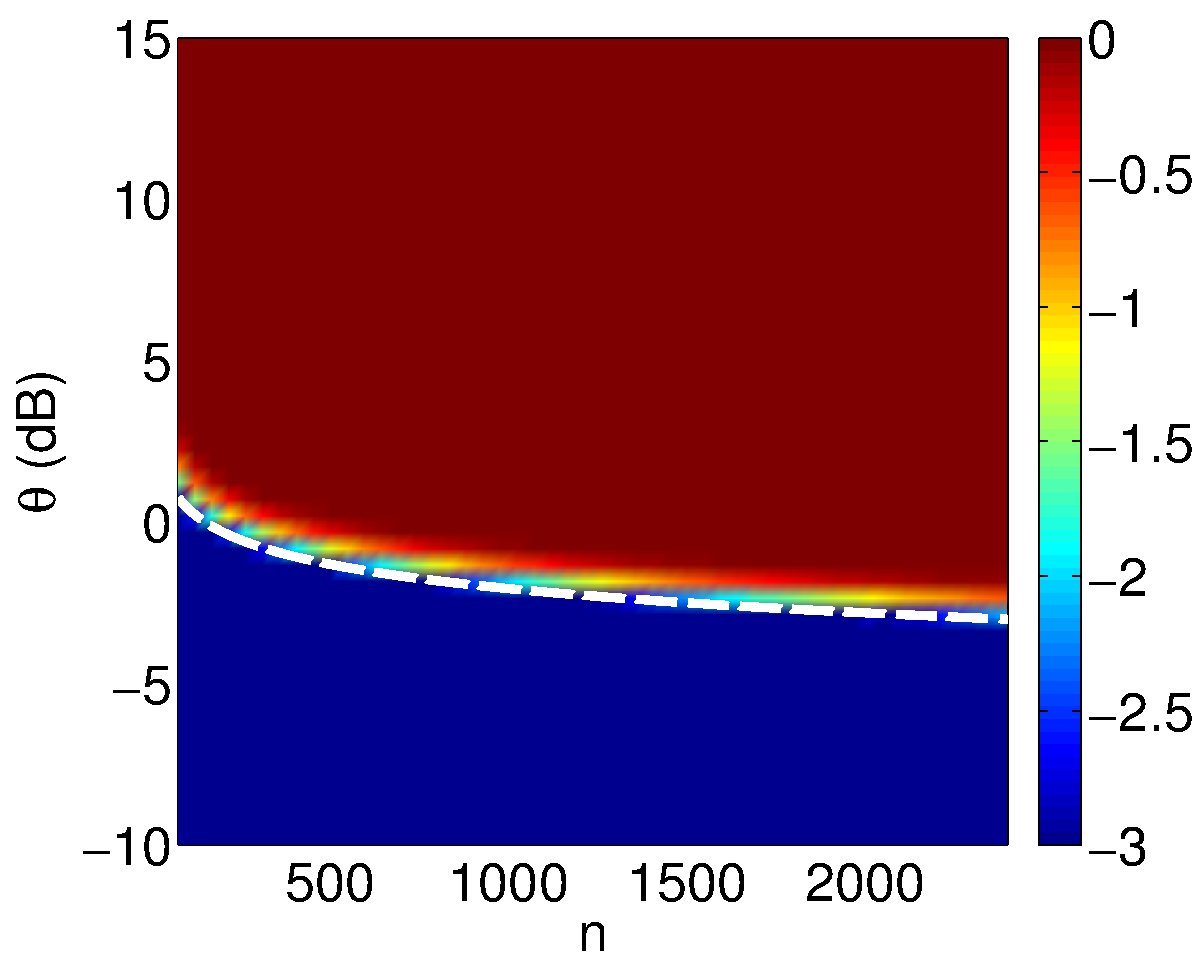
\includegraphics[width=0.35\textwidth]{figures/icca_rho9.pdf}
    \end{center}

  \end{column}
  \end{columns}



\end{frame}

%%%%%%%%%%%%%%%%%%%%%%%%%%%%%%%%%%%%%%%%%%%%%
\begin{frame}{Empirical CCA and ICCA Demonstration}
%      \textbf{ICCA Correlations}\hspace{20ex}\textbf{Significance}

  \begin{columns}[T]
  \begin{column}{0.01\textwidth}
    \vspace{15ex}
    \textbf{Correlations}\\
    \vspace{20ex}
    \textbf{Significance}
  \end{column}
  \begin{column}{1\textwidth}
    \begin{center}
      \href{run:/home/asendorf/Documents/thesis_videos/flashing_video2.mp4}{\textbf{Video-Video}}\hspace{20ex}\href{run:/home/asendorf/Documents/thesis_videos/av_coffee_pres.mp4}{\textbf{Audio-Video}}\\
        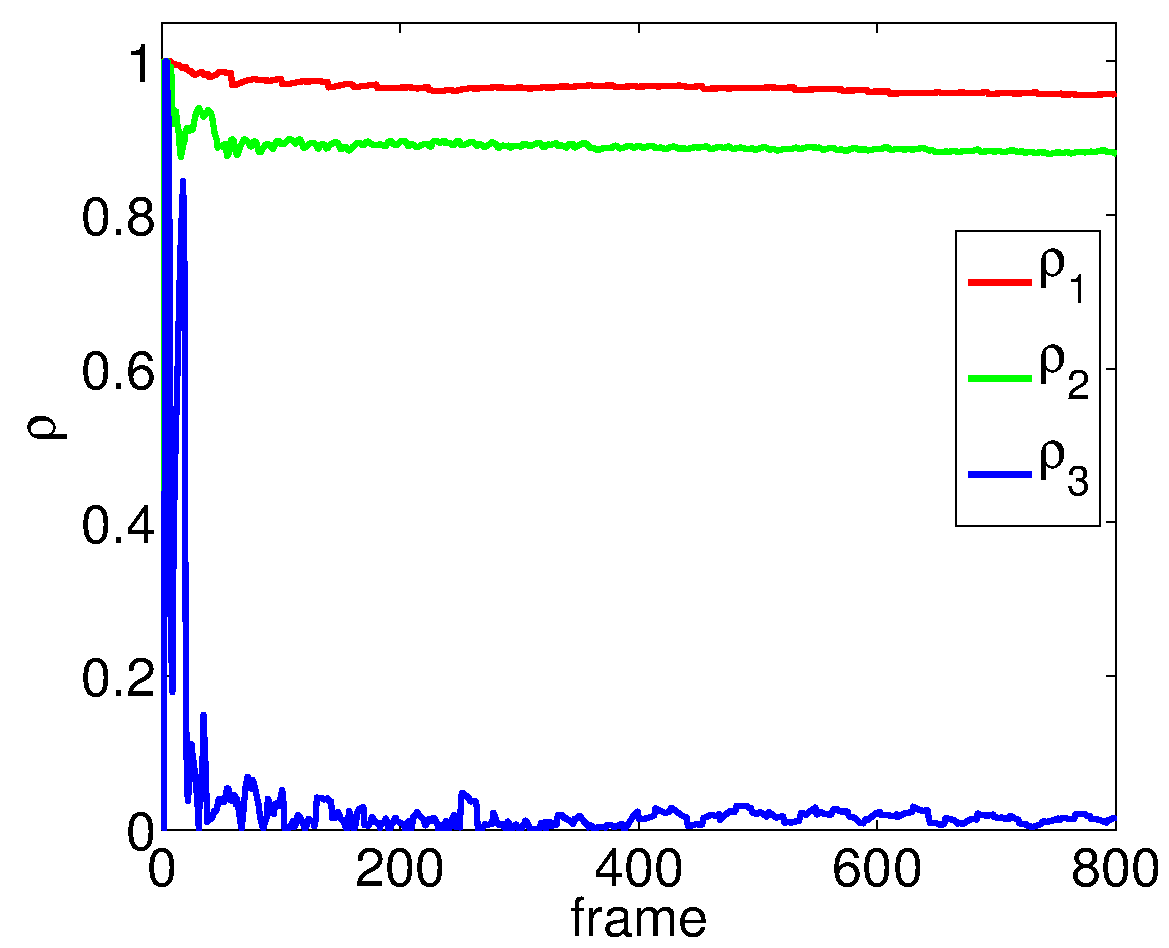
\includegraphics[width=0.38\textwidth]{figures/flashing_icca_corrs.pdf}
        \hspace{2ex}
        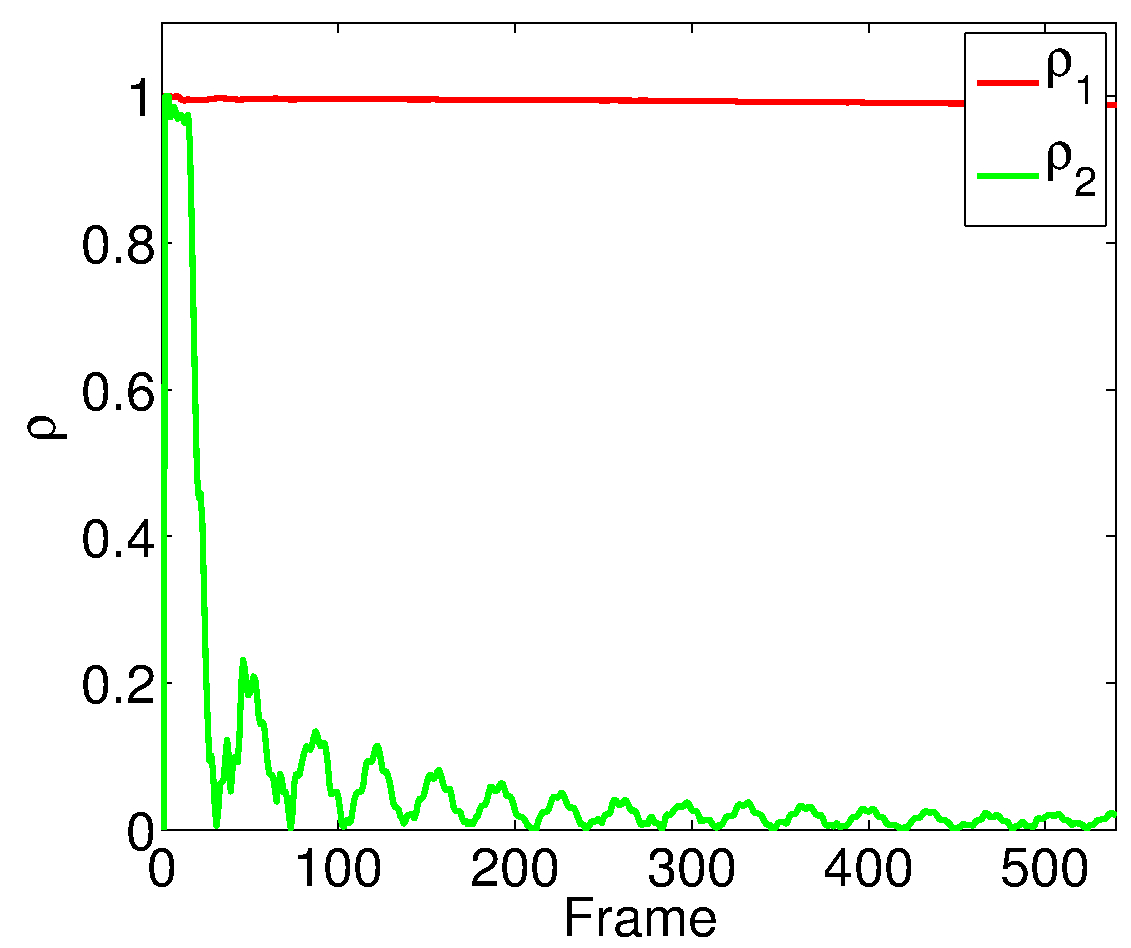
\includegraphics[width=0.38\textwidth]{figures/av_icca_corrs.pdf}\\[2ex]
        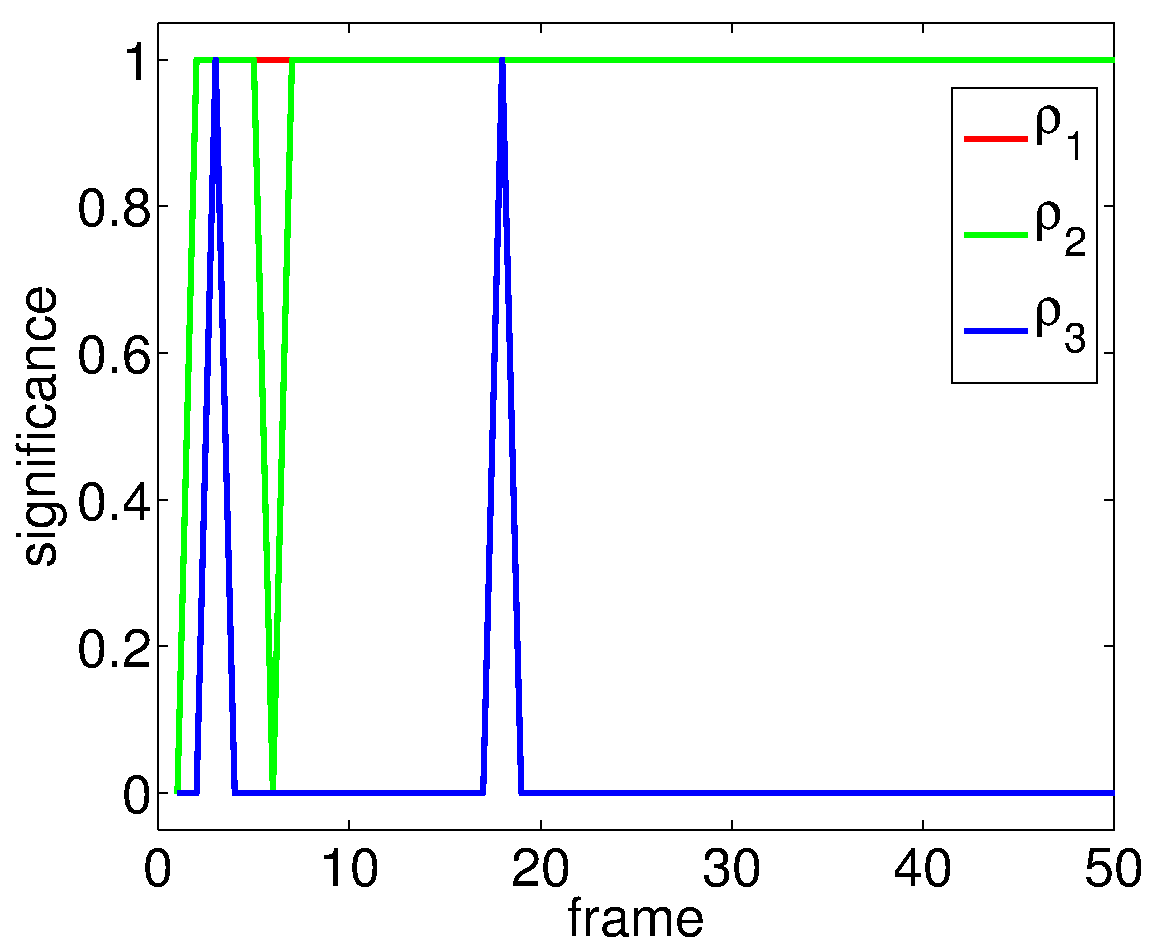
\includegraphics[width=0.38\textwidth]{figures/flashing_icca_sig_zoom.pdf}
        \hspace{2ex}
        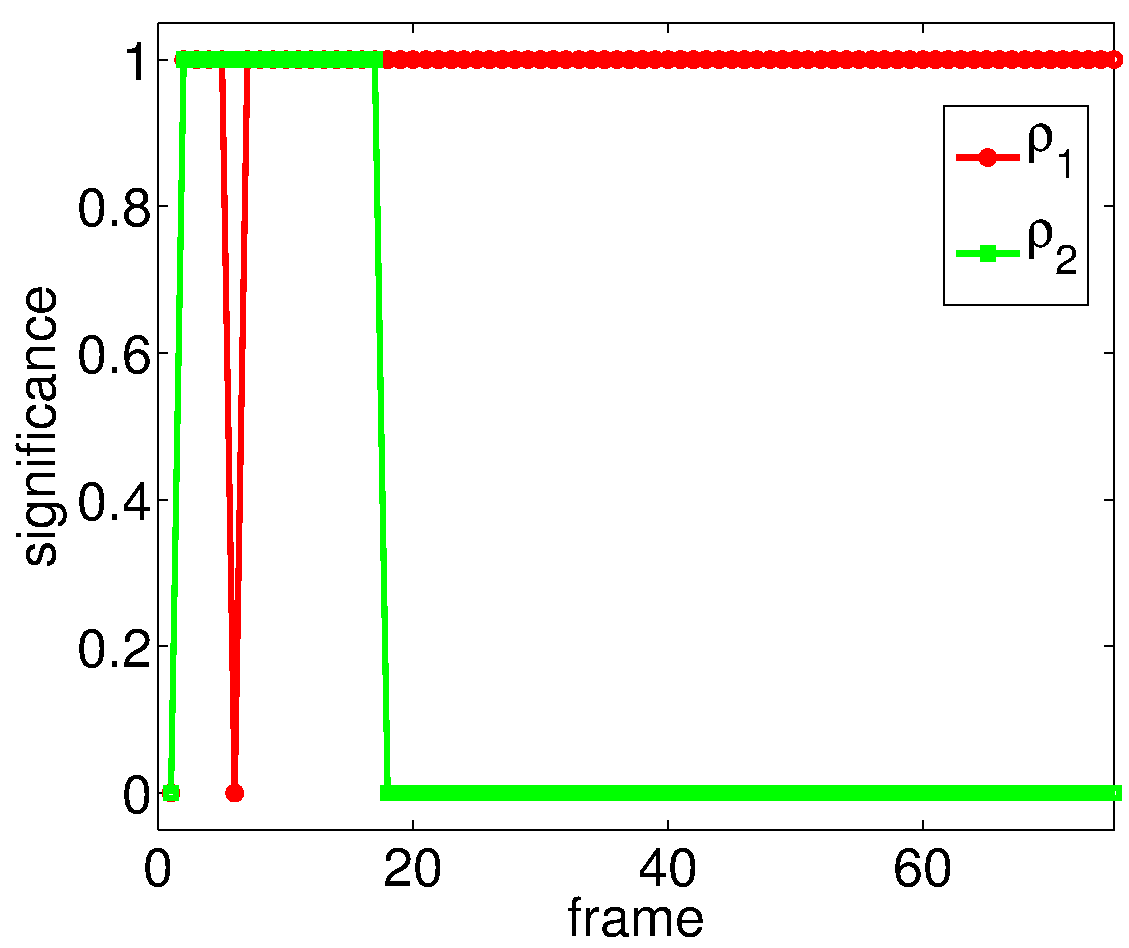
\includegraphics[width=0.38\textwidth]{figures/av_icca_sig_zoom.pdf}
    \end{center}
  \end{column}
  \end{columns}


\end{frame}

%%%%%%%%%%%%%%%%%%%%%%%%%%%%%%%%%%%%%%%%%%%%%%%%%%%%%%%%%%%%%%%%%%%%%%%%%%%%%%
\begin{frame}{Correlation Analysis Wish List}
  \addtocounter{framenumber}{-1}

  \begin{center}
    \textbf{Correlation Algorithm Wish List}\\[1ex]
\fcolorbox{black}[HTML]{F1F1F1}{\parbox{0.8\textwidth}{%
    \begin{enumerate}
    \item \textbf{Reliable in the sample deficient regime}
      \begin{itemize}
      \item {\textcolor{texthigh}{meaningful correlations \checkmark}}
      \item meaningful canonical vectors
      \end{itemize}
    \item {\textcolor{texthigh}{\textbf{Statistical test for correlations} \checkmark}}
      \begin{itemize}
      \item {\textcolor{texthigh}{consistency analysis \checkmark}}
      \end{itemize}
    \item \textbf{Robust}
      \begin{itemize}
      \item non-gaussian data
      \item missing data
      \end{itemize}
    \item \textbf{Extends to more than 2 datasets}
    \end{enumerate}
}}
\end{center}

\end{frame}

%%%%%%%%%%%%%%%%%%%%%%%%%%%%%%%%%%%%%%%%%%%%%%%%%%%%%%%%%%%%%%%%%%%%%%%%%%%%
\begin{frame}{Missing Data Model}

\textbf{Matrix model}
\begin{itemize}
\item $V_x = \left[s_{x,1},\dots,s_{x,n}\right]$, $V_y = \left[s_{y,1},\dots,s_{y,n}\right]$
\item $Z_x = \left[z_{x,1},\dots,z_{x,n}\right]$, $Z_y = \left[z_{y,1},\dots,z_{y,n}\right]$
\end{itemize}

\vspace{2ex}

\begin{center}
\fcolorbox{black}[HTML]{F1F1F1}{\parbox{0.5\textwidth}{
    \be\ba
    & X = \left(U_xV_x^H + Z_x\right)\odot M_x\\
    & Y = \left(U_yV_y^H + Z_y\right)\odot M_y\\
    \ea\ee
  }}
\end{center}

\be\ba
& M^x_{ij} = \begin{cases} 1 & \text{ with probability } \gamma_x\\ 0 & \text{ with
    probability } 1-\gamma_x \end{cases}
& M^y_{ij} = \begin{cases} 1 & \text{ with probability } \gamma_y\\ 0 & \text{ with
    probability } 1-\gamma_y \end{cases}
\ea\ee
\begin{itemize}
\item $\odot$ denotes the Hadamard or element-wise product.
\end{itemize}
\end{frame}

%%%%%%%%%%%%%%%%%%%%%%%%%%%%%%%%%%%%%%%%%%%%%%%%%%%%%%%%%%%%%%%%%%%%%%%%%%%%
\begin{frame}{Empirical CCA and ICCA Consistency in Missing Data}

\begin{Th}[Missing data consistency]\label{th:missing_data}
Let $p,q,n\to\infty$ with $p/n\to c_x$ and $q/n\to c_y$ and assume a low-coherence
condition on the signal vectors. Given a linear subspace data model with missing data
entries, 
\be\ba
& \widehat{k}_{\text{cca}} \convas k &&\text{ if } \min_{i=1,\dots,k}\kapcir_i^2 >r_c \text{ and } n>p+q\\
& \widehat{k}_{\text{icca}} \convas k && \text{ if } \min_{i=1,\dots,\widehat{k}_x}
\theta_i^{(x)}>\frac{c_x^{1/4}}{\sqrt{\gamma_x}} \text{ and } 
\min_{i=1,\dots,\widehat{k}_y} \theta_i^{(y)}>\frac{c_y^{1/4}}{\sqrt{\gamma_y}}
\ea\ee
where $\kapcir_i$ are the singular values of 
\be
\left(\gamma_x\Theta_x+I_{k_x}\right)^{-1/2}\left(\gamma_x\Theta_x\right)^{1/2}P_{xy}\left(\gamma_y\Theta_y\right)^{1/2}
\left(\gamma_y\Theta_y+I_{k_y}\right)^{-1/2}.
\ee
\end{Th}

\end{frame}

%%%%%%%%%%%%%%%%%%%%%%%%%%%%%%%%%%%%%%%%%%%%%%%%%%%%%%%%%%%%%%%%%%%%%%%%%%%%
\begin{frame}{Empirical CCA and ICCA Consistency in Missing Data}

  \begin{itemize}
  \item $p=q=150$, $n=1200$, $k=1$, $\theta=\theta_x=\theta_y$,$\alpha=0.01$
  \end{itemize}

  \begin{columns}[T]
    \begin{column}{0.01\textwidth}
      \vspace{15ex}
      \textbf{ CCA}\\
      \vspace{20ex}
      \textbf{ICCA}
    \end{column}
    \begin{column}{1\textwidth}
      \begin{center}
        $\boldsymbol{\rho=}\mathbf{0.7}$\hspace{22ex}$\boldsymbol{\rho=0.9}$\\[0.5ex]
        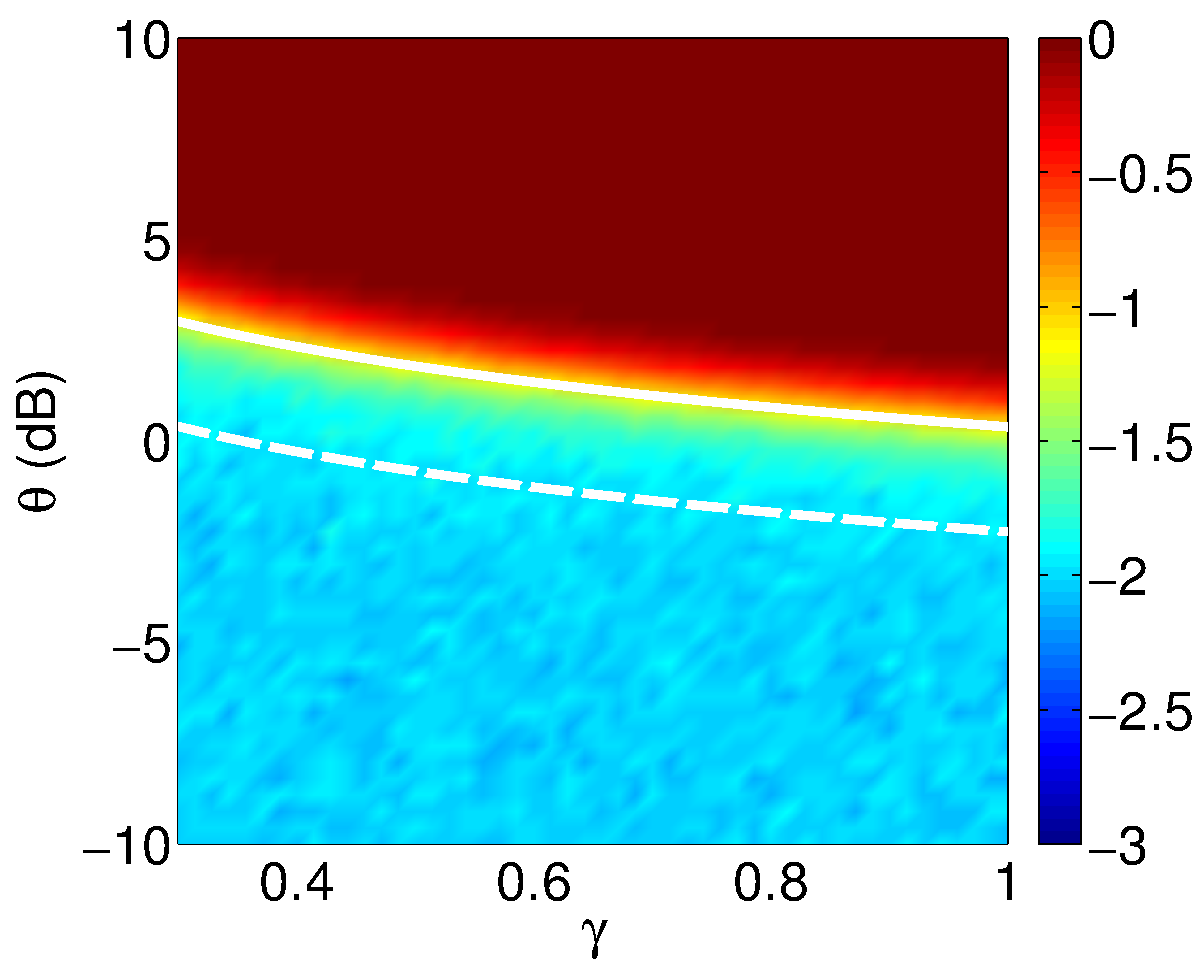
\includegraphics[width=0.35\textwidth]{figures/cca_missing_7_1200.pdf}\hspace{2ex}
        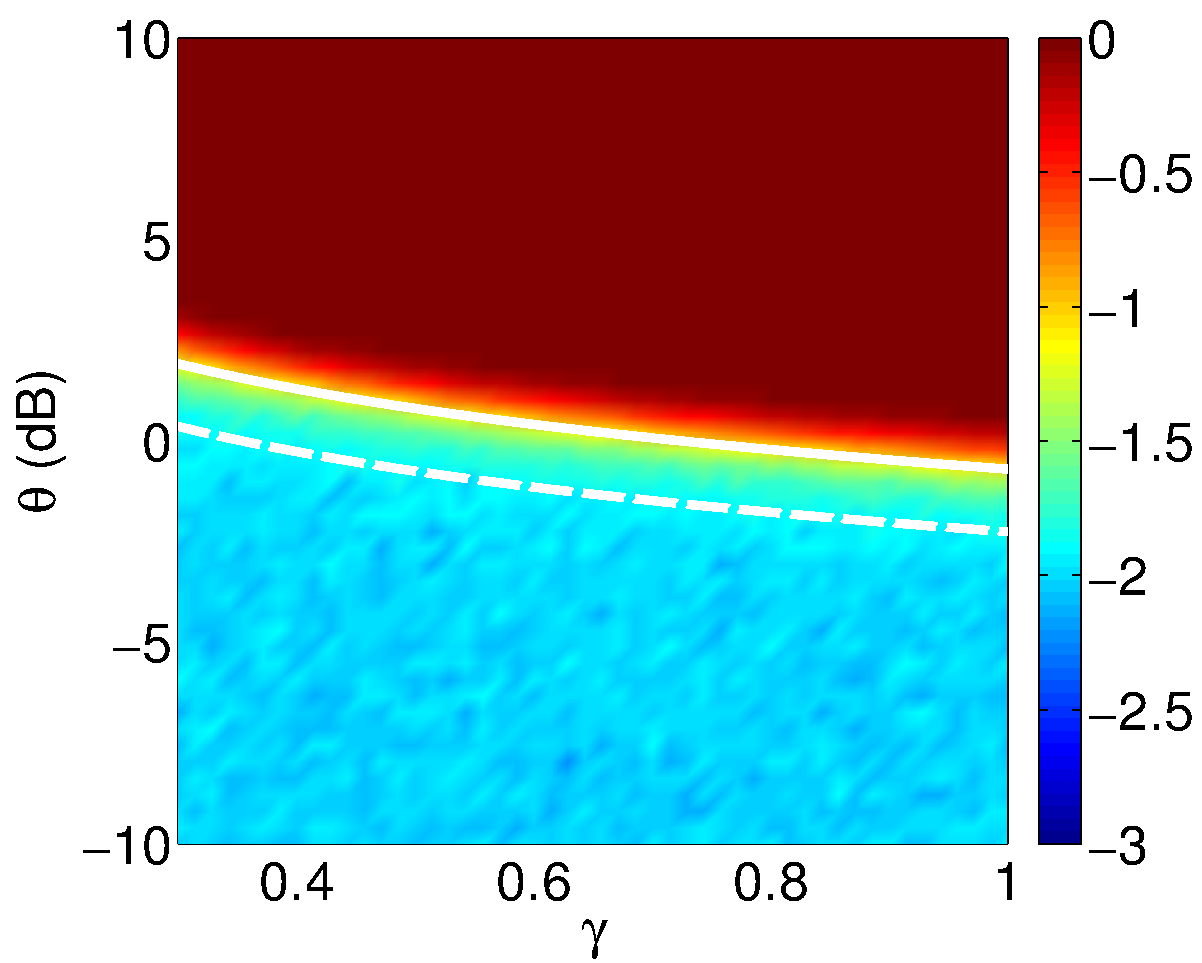
\includegraphics[width=0.35\textwidth]{figures/cca_missing_9_1200.pdf}\\[2ex]
        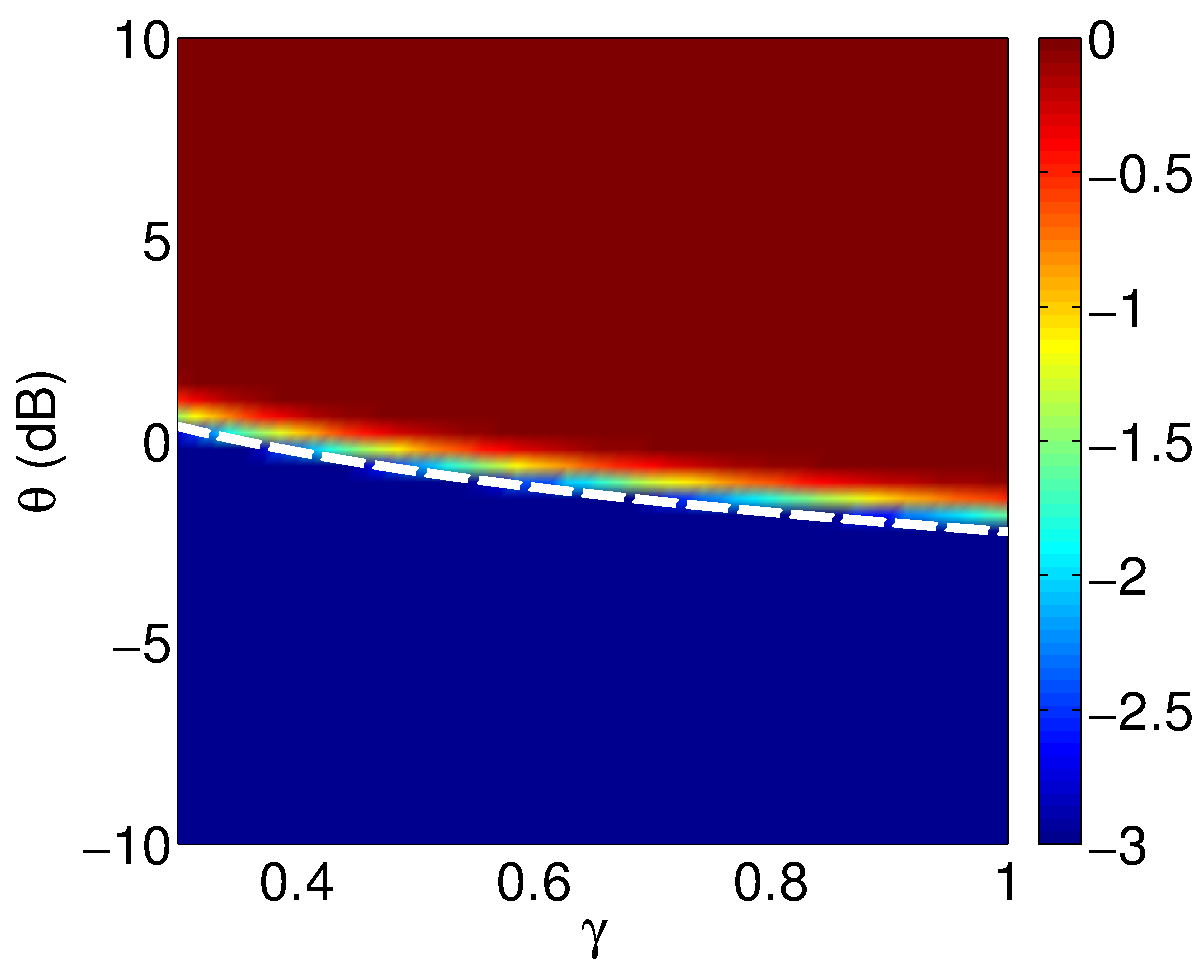
\includegraphics[width=0.35\textwidth]{figures/icca_missing_7_1200.pdf}\hspace{2ex}
        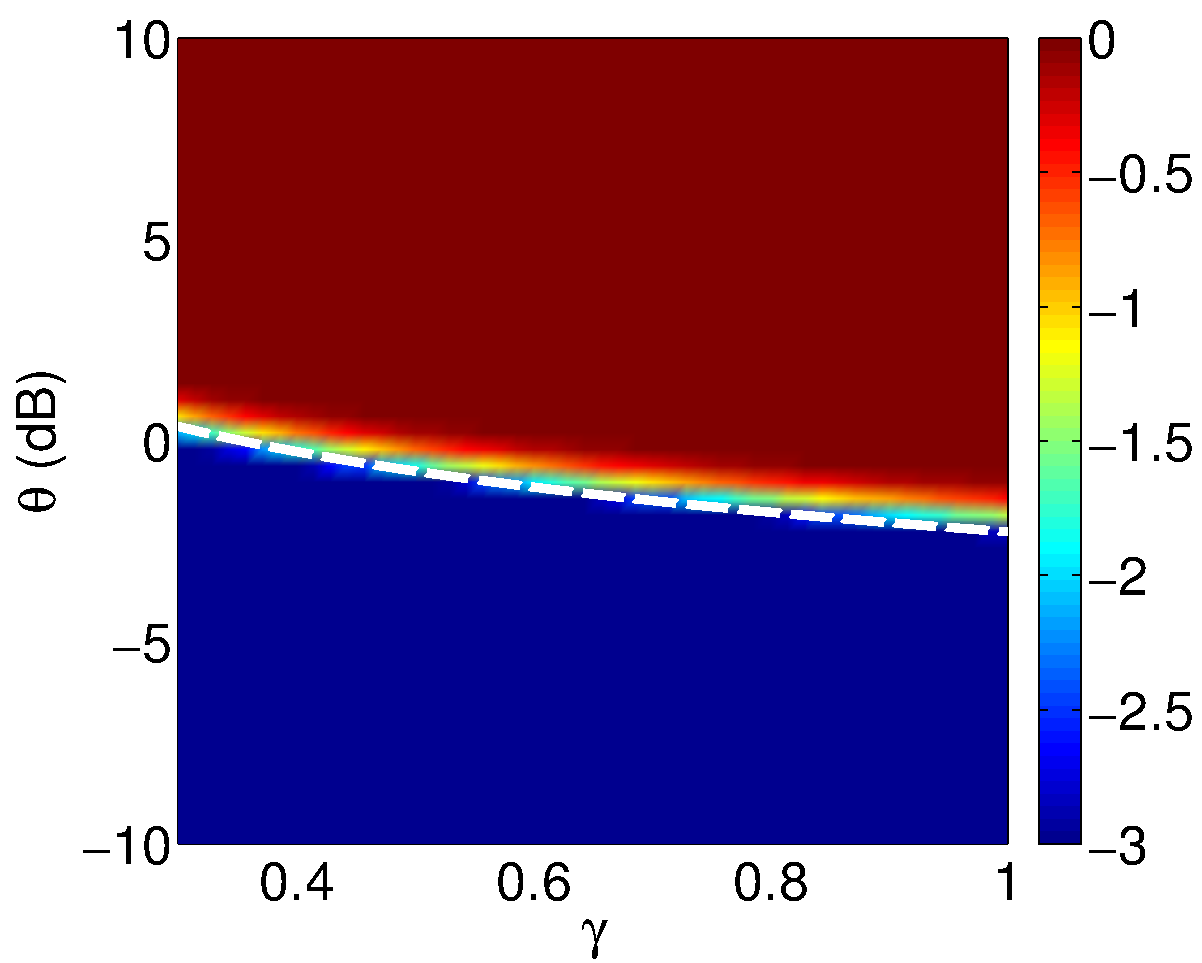
\includegraphics[width=0.35\textwidth]{figures/icca_missing_9_1200.pdf}
      \end{center}
    \end{column}
  \end{columns}

\end{frame}

%%%%%%%%%%%%%%%%%%%%%%%%%%%%%%%%%%%%%%%%%%%%%%%%%%%%%%%%%%%%%%%%%%%%%%%%%%%%%%
\begin{frame}{\href{run:/home/asendorf/Documents/thesis_videos/youtube_missing.mp4}{Missing Data
      Demonstration}}

  \begin{itemize}
  \item $p=q=32400$ pixels
  \item $n=600$ frames
  \item $\gamma_x=\gamma_y=0.75$
  \end{itemize}

  \vspace{3ex}

  \begin{center}
    \textbf{ICCA Correlations}\hspace{23ex}\textbf{Significance}\\[0.5ex]
    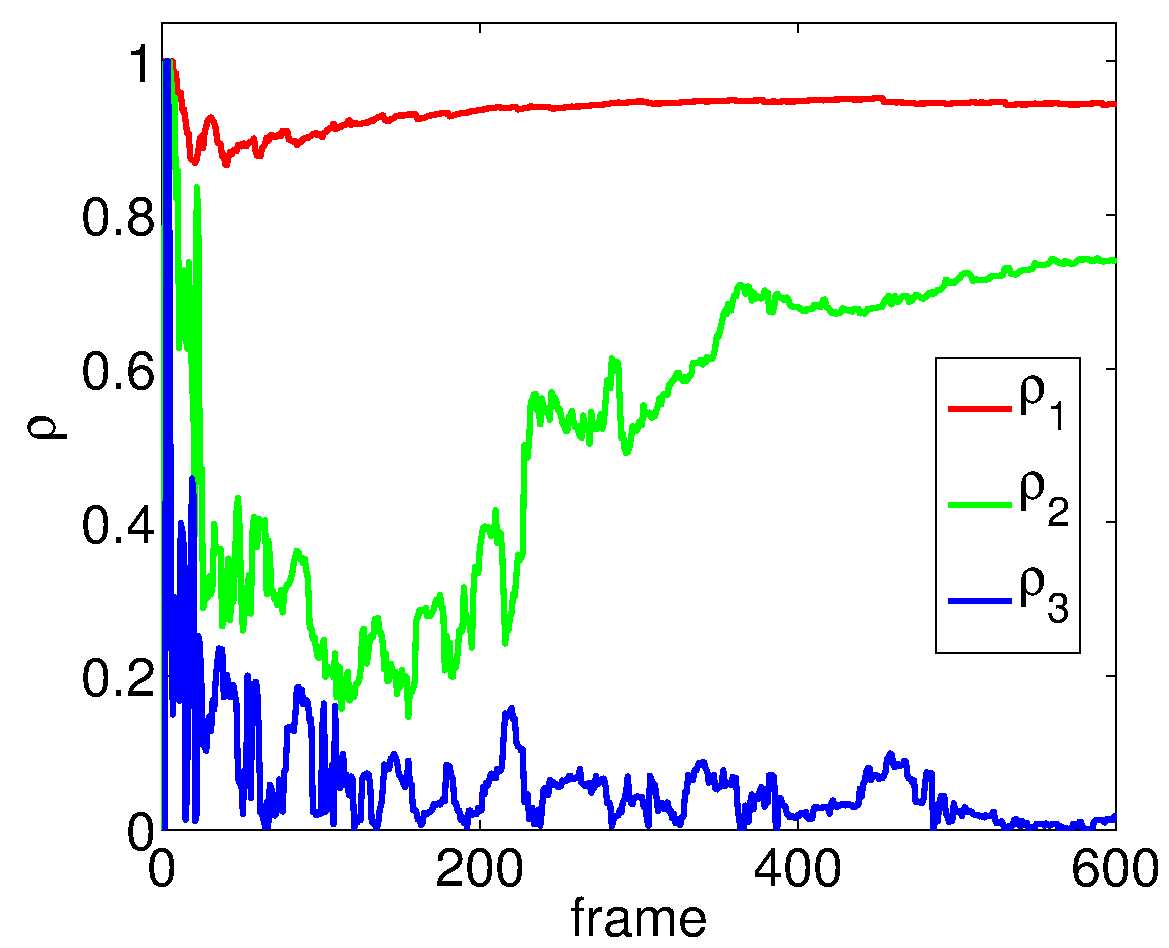
\includegraphics[width=0.45\textwidth]{figures/icca_corrs_miss.pdf}\hspace{2ex}
    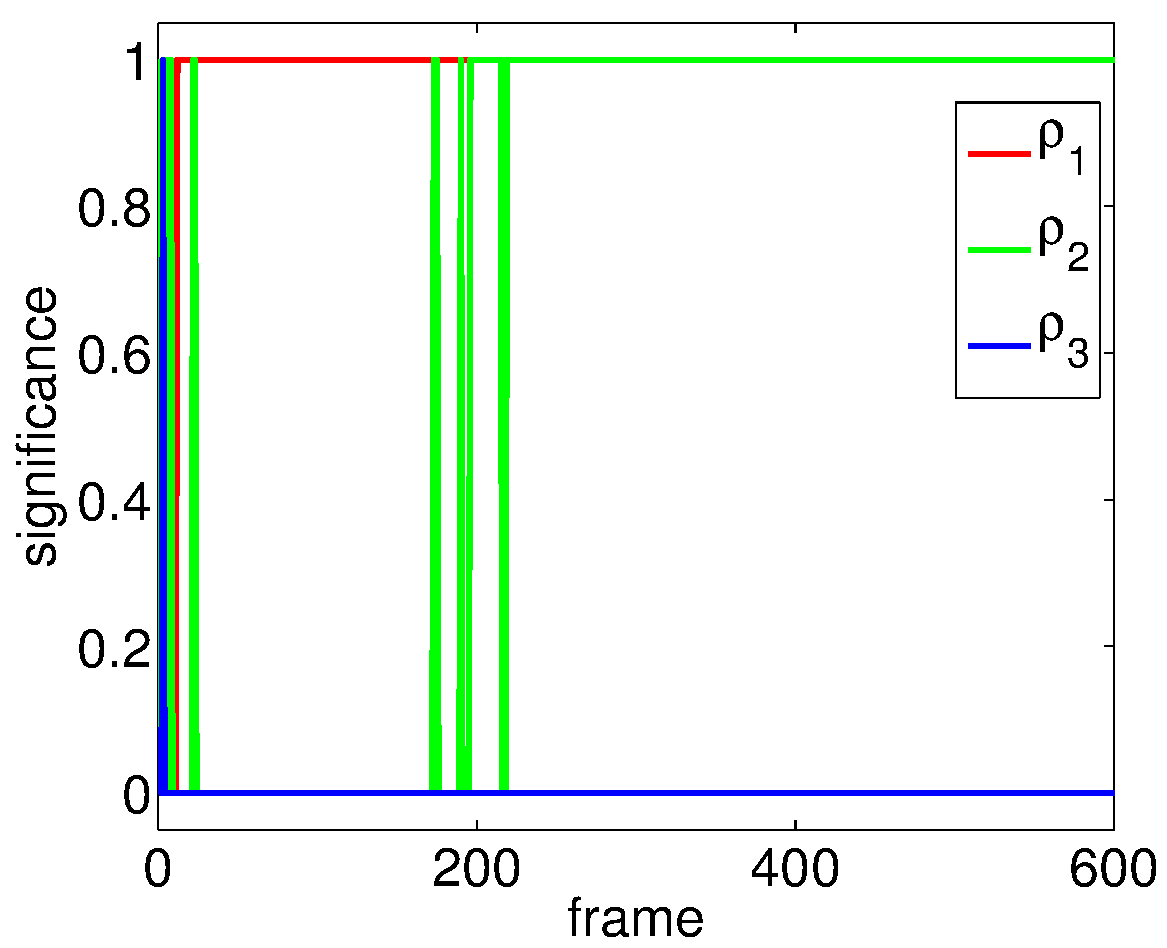
\includegraphics[width=0.45\textwidth]{figures/icca_sigs_miss.pdf}\\[2ex]
  \end{center}

\end{frame}

%%%%%%%%%%%%%%%%%%%%%%%%%%%%%%%%%%%%%%%%%%%%%%%%%%%%%%%%%%%%%%%%%%%%%%%%%%%%%%
\begin{frame}{Non-Gaussian Data}

  \textbf{Relax Noise Assumptions}
  \begin{itemize}
  \item $\zx$ and $\zy$ are zero mean with bounded fourth moment
  \end{itemize}
  \vspace{2ex}
  \begin{center}
    \textbf{ICCA consistency theorem still holds}\\[0.5ex]
    \fcolorbox{black}[HTML]{F1F1F1}{\parbox{0.8\textwidth}{
        \be
        \widehat{k}_{\text{icca}} \convas k \text{ if } \min_{i=1,\dots,\widehat{k}_x}
        \theta_i^{(x)}>c_x^{1/4} \text{ and } \min_{i=1,\dots,\widehat{k}_y}
        \theta_i^{(y)}>c_y^{1/4} 
        \ee
      }}
  \end{center}
  \vspace{2ex}
  \textbf{General Form}
  \begin{itemize}
  \item $\zx$ and $\zy$ are drawn from noise distributions $\mu_{Z_x}$ and $\mu_{Z_y}$
  \item consistency dependent on D-transforms of noise distributions
  \end{itemize}



%\begin{Corr}[Non-Gaussian Data]
%  Let $\mu_{Z_x}$ and $\mu_{Z_y}$ be the
%  non-random compactly supported probability measures modeling the singular values of the
%  noise matrices $X$ and $Y$. Let $b_x$ and $b_y$ be the supremums of the supports,
%  respectively. Let $p,q,n\to\infty$ with $p/n\to c_x$ and $q/n\to c_y$. ICCA returns a
%  consistent estimate of the number of correlated components under the following conditions
%  \be
%  \khaticca \convas k \text{ if } \min_{i=1,\dots,\kx}\tx_i>\frac{1}{D_{\mu_{Z_x}}(b_x^+)}
%  \text{ and } \min_{i=1,\dots,\ky}\ty_i > \frac{1}{D_{\mu_{Z_y}}(b_y^+)}
%  \ee
%  where $D_{\mu_x}$ and $D_{\mu_y}$, the D-transforms of $\mu_{Z_x}$ and $\mu_{Z_y}$, are the
%  functions, depending on $c_x$ and $c_y$.
%\end{Corr}

\end{frame}



%%%%%%%%%%%%%%%%%%%%%%%%%%%%%%%%%%%%%%%%%%%%%%%%%%%%%%%%%%%%%%%%%%%%%%%%%%%%%%
\begin{frame}{Correlation Analysis Wish List}
  \addtocounter{framenumber}{-1}

  \begin{center}
    \textbf{Correlation Algorithm Wish List}\\[1ex]
\fcolorbox{black}[HTML]{F1F1F1}{\parbox{0.8\textwidth}{%
    \begin{enumerate}
    \item \textbf{Reliable in the sample deficient regime}
      \begin{itemize}
      \item {\textcolor{texthigh}{meaningful correlations \checkmark}}
      \item meaningful canonical vectors
      \end{itemize}
    \item {\textcolor{texthigh}{\textbf{Statistical test for correlations} \checkmark}}
      \begin{itemize}
      \item {\textcolor{texthigh}{consistency analysis \checkmark}}
      \end{itemize}
    \item {\textcolor{texthigh}{\textbf{Robust} \checkmark}}
      \begin{itemize}
      \item {\textcolor{texthigh}{non-gaussian data \checkmark}}
      \item {\textcolor{texthigh}{missing data \checkmark}}
      \end{itemize}
    \item \textbf{Extends to more than 2 datasets}
    \end{enumerate}
}}
\end{center}

\end{frame}


%%%%%%%%%%%%%%%%%%%%%%%%%%%%%%%%%%%%%%%%%%%%%%%%%%%%%%%%%%%%%%%%%%%%%%%
\begin{frame}{MCCA - Multiset CCA}

  \begin{center}
    \fcolorbox{black}[HTML]{F1F1F1}{\parbox{0.6\textwidth}{%
        \centering What if we have $m$ datasets $Y_1,\dots,Y_m$?  }}
  \end{center}

\vspace{1ex}

\textbf{Notation}
\begin{itemize}
\item covariance matrices: $R_{ij} = \E{y_iy_j^H}$
\item canonical vectors: $x_1,\dots,x_m$
\item canonical variates: $w_1,\dots, w_m$, $w_i=x_i^Hy_i$
\end{itemize}

\vspace{2ex}

\begin{equation*}
\Phi(x)=E[ww^H]=\left[\begin{array}{ccc} x_1^HR_{11}x_1 & \dots & x_1^HR_{1m}x_m \\ \vdots
    & \ddots & \vdots \\ x_m^HR_{m1}x_1 & \dots & x_m^HR_{mm}x_m\\ \end{array}\right]
\end{equation*}

\vspace{1ex}

\begin{center}
  \textbf{Optimization Problem}\\

  \fcolorbox{black}[HTML]{F1F1F1}{\parbox{0.5\textwidth}{%
      \be\ba
      &\underset{x}{\mathop{\rm optimize}} && J(\Phi(x))\\
      &\mathop{\rm subject~ to} && h(x,R)\\
      \ea\ee
    }}
\end{center}


\end{frame}

%%%%%%%%%%%%%%%%%%%%%%%%%%%%%%%%%%%%%%%%%%%%%
\begin{frame}{MCCA - Maximum Variance (MAXVAR)}

  \begin{center}
    \textbf{MAXVAR Optimization Problem}\\
    \fcolorbox{black}[HTML]{F1F1F1}{\parbox{0.4\textwidth}{%
        \be\ba
        &\argmax_{x_1,\dots,x_m}&&\lambda_1\left(\Phi(x)\right)\\
        &\text{subject to} &&x_i^HR_{ii}x_i = 1
        \ea\ee
      }}
  \end{center}

  \vspace{1ex}

  \textbf{Empirical MAXVAR}
  \begin{itemize}
  \item Let $V_i$ be the right singular vectors of dataset $Y_i$
  \item $\lambda_j\left(\widehat{\Phi}(x)\right) = \lambda_j\left(\Cmccahat\right)$
    \end{itemize}

    \be
    \Cmccahat=\left[\begin{array}{cccc} I_{d_1} & V_1^HV_2 & \cdots & V_1^HV_m\\
        V_2^HV_1 & I_{d_2} & \cdots & V_2^HV_m\\
        \vdots & \vdots & \ddots & \vdots\\
        V_m^HV_1 & V_m^HV_2 & \cdots & I_{d_m}\end{array}\right]
    \ee

    \vspace{2ex}

      \begin{center}
        \textbf{Proposed correlation statistic}\\
        \fcolorbox{black}[HTML]{F1F1F1}{\parbox{0.4\textwidth}{%
            \be
            \widehat{\rho}^{(j)}_{\text{mcca}} = \lambda_j\left(\Cmccahat - I\right)
            \ee
          }}
      \end{center}


\end{frame}

%%%%%%%%%%%%%%%%%%%%%%%%%%%%%%%%%%%%%%%%%%%%%
\begin{frame}{Informative MCCA}

  \textbf{Idea - Trim right singular vectors}
  \begin{itemize}
  \item  $\Vcir_i = \widehat{V}_i\left(:,1:\widehat{k}_i\right)$
  \item  $\Vcir =\left[\Vcir_1,\dots \Vcir_m\right]$
  \end{itemize}

  \begin{columns}[t]
    \begin{column}{0.5\textwidth}
      \begin{center}
        \textbf{New IMCCA Matrix}\\
        \fcolorbox{black}[HTML]{F1F1F1}{\parbox{0.8\textwidth}{%
            \be
            \Cimccahat = \Vcir^H\Vcir
            \ee
          }}
      \end{center}
    \end{column}
    \begin{column}{0.5\textwidth}
      \begin{center}
        \textbf{Proposed correlation statistic}\\
        \fcolorbox{black}[HTML]{F1F1F1}{\parbox{0.8\textwidth}{%
            \be
            \widehat{\rho}^{(j)}_{\text{imcca}} = \lambda_j\left(\Cimccahat - I\right)
            \ee
          }}
      \end{center}
    \end{column}
  \end{columns}

  \vspace{2ex}

  \textbf{Insights}
  \begin{itemize}
  \item Eigenvalue detects correlation
  \item Eigenvector reveals structure
  \end{itemize}


\end{frame}

%%%%%%%%%%%%%%%%%%%%%%%%%%%%%%%%%%%%%%%%%%%%%
\begin{frame}{\href{run:/home/asendorf/Documents/thesis_videos/mcca_flashing.mp4}{Empirical
      MCCA and
      IMCCA Demonstration}} 

    \begin{center}
      \hspace{-3ex}\textbf{Empirical MCCA Correlations}\hspace{13ex}\textbf{IMCCA Correlations}
        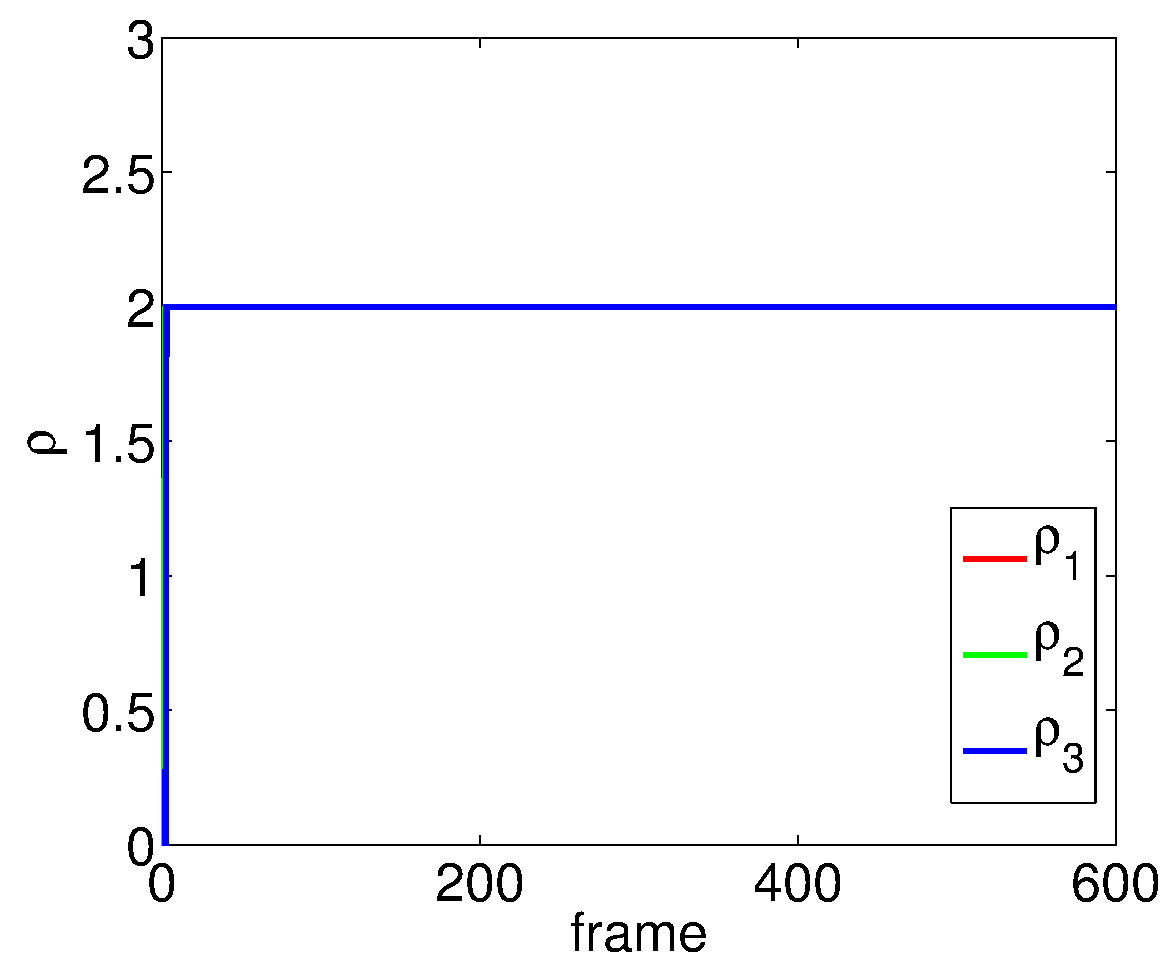
\includegraphics[width=0.45\textwidth]{figures/mcca_cca_corrs.pdf}\hspace{2ex}
        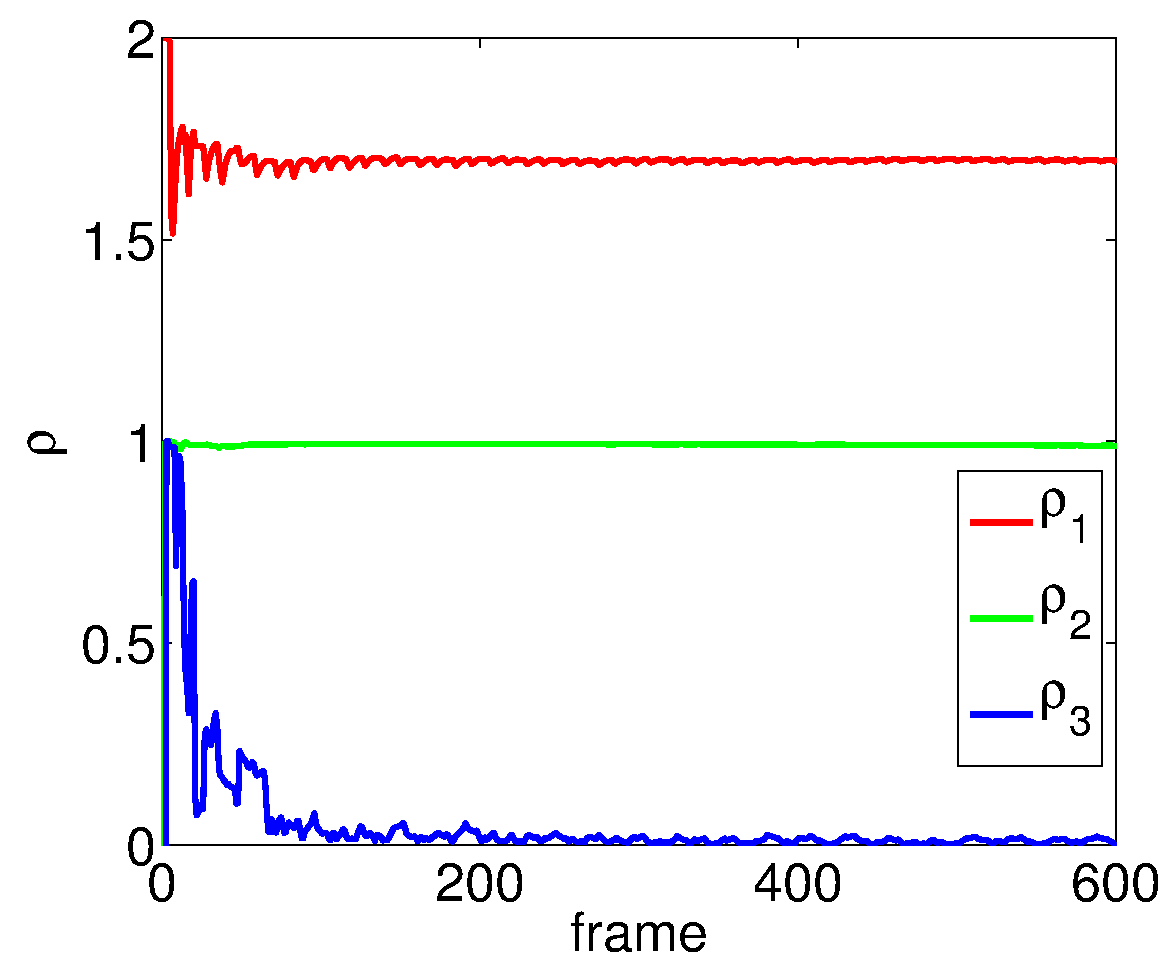
\includegraphics[width=0.45\textwidth]{figures/mcca_icca_corrs.pdf}
    \end{center}

\end{frame}

%%%%%%%%%%%%%%%%%%%%%%%%%%%%%%%%%%%%%%%%%%%%%%%%%%%%%%%%%%%%%%%%%%%%%%%%%%%%%%
\begin{frame}{Correlation Analysis Wish List}
  \addtocounter{framenumber}{-1}

  \begin{center}
    \textbf{Correlation Algorithm Wish List}\\[1ex]
\fcolorbox{black}[HTML]{F1F1F1}{\parbox{0.8\textwidth}{%
    \begin{enumerate}
    \item \textbf{Reliable in the sample deficient regime}
      \begin{itemize}
      \item {\textcolor{texthigh}{meaningful correlations \checkmark}}
      \item meaningful canonical vectors
      \end{itemize}
    \item {\textcolor{texthigh}{\textbf{Statistical test for correlations} \checkmark}}
      \begin{itemize}
      \item {\textcolor{texthigh}{consistency analysis \checkmark}}
      \end{itemize}
    \item {\textcolor{texthigh}{\textbf{Robust} \checkmark}}
      \begin{itemize}
      \item {\textcolor{texthigh}{non-gaussian data \checkmark}}
      \item {\textcolor{texthigh}{missing data \checkmark}}
      \end{itemize}
    \item \textcolor{texthigh}{\textbf{Extends to more than 2 datasets} \checkmark}
    \end{enumerate}
}}
\end{center}

\end{frame}


%%%%%%%%%%%%%%%%%%%%%%%%%%%%%%%%%%%%%%%%%%%%%%%%%%%%%%%%%%%%%%%%%%%%%%%%%%%%%%
\begin{frame}{Canonical Vector Estimation - Chpt. 5}

\textbf{Data SVDs}
\begin{itemize}
\item $X=\Uxhat\Sigxhat\Vxhat^H$ with trimmed versions $\Uxcir$, $\Sigxcir$, $\Vxcir$
\item $\Uktil$ left singular vectors of $\Kxytil$
\item $\widehat{U}_{\widetilde{K}}$ left singular vectors of $\Cccahat$
\item $\Ukcir$ left singular vectors of $\Ciccahat$
\end{itemize}

\vspace{3ex}

\begin{table}[t]
\centering
\begin{tabular}{l|l}\toprule
Estimate & \\
\midrule
\textbf{Population}  & $W_x = \Ux\left(\Tx + I_{\kx}\right)^{-1/2}\Uktil$\\[1ex]
\textbf{Empirical CCA} & $\widehat{W}_x^{\text{cca}} =
\Uxhat\left(\Sigxhat\right)^{-1}\widehat{U}_{\widetilde{K}}$\\[1ex]
\textbf{ICCA} & $\widehat{W}_x^{\text{icca}} = \Uxcir\Sigxcir^{-1}\Ukcir$\\[1ex]
\textbf{\iccap} &$\widehat{W}_x^{\text{icca+}} = \Uxcir\Lambda_x^{\text{opt}}\Ukcir$\\[1ex]
\bottomrule
\end{tabular}
\end{table}

\end{frame}


%%%%%%%%%%%%%%%%%%%%%%%%%%%%%%%%%%%%%%%%%%%%%%%%%%%%%%%%%%%%%%%%%%%%%%%%%%%%%% 
\begin{frame}{Canonical Vector Accuracy Experiment}

\begin{columns}[T]
  \begin{column}{0.3\textwidth}
    \vspace{15ex}
    \begin{center}
    \textbf{Original Scene}
    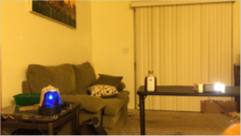
\includegraphics[width=\textwidth]{figures/flashing_left.png}
\end{center}
  \end{column}
  \begin{column}{0.7\textwidth}
    \begin{center}
      \textbf{ICCA}\hspace{20ex}\textbf{\iccap}\phantom{blah}\\
      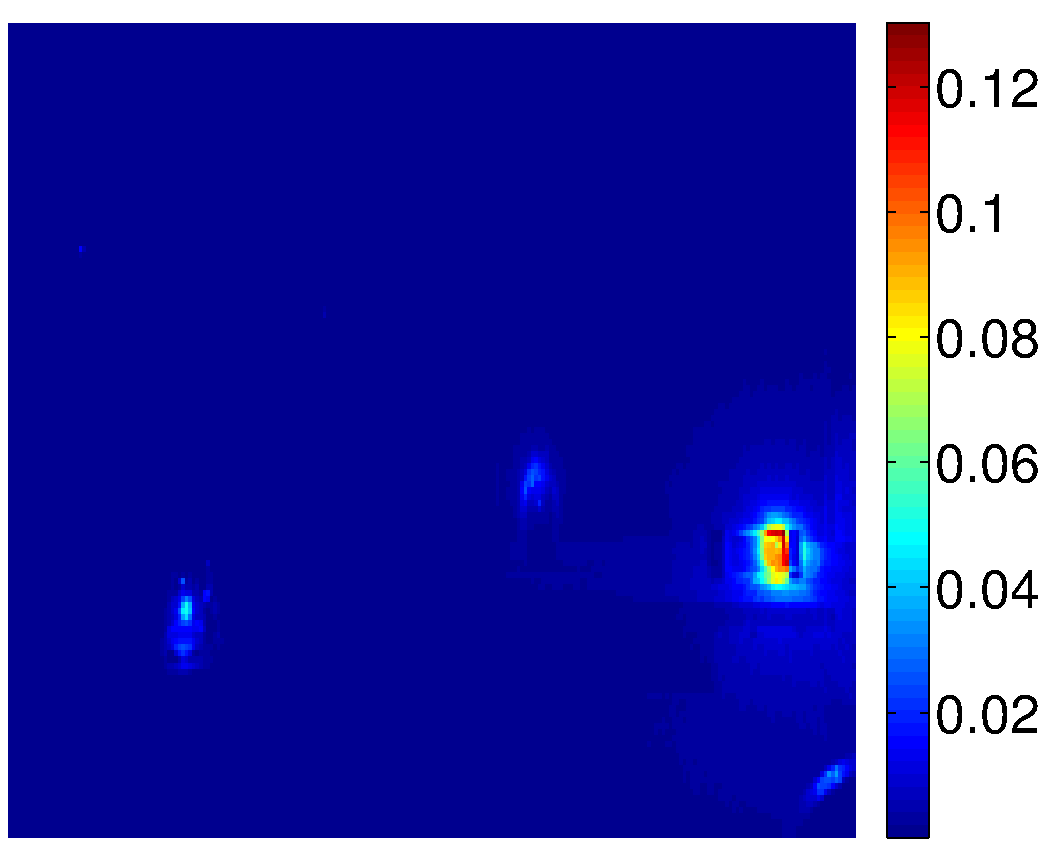
\includegraphics[width=0.45\textwidth]{figures/flashing1_left1_icca.pdf}\hspace{2ex}
      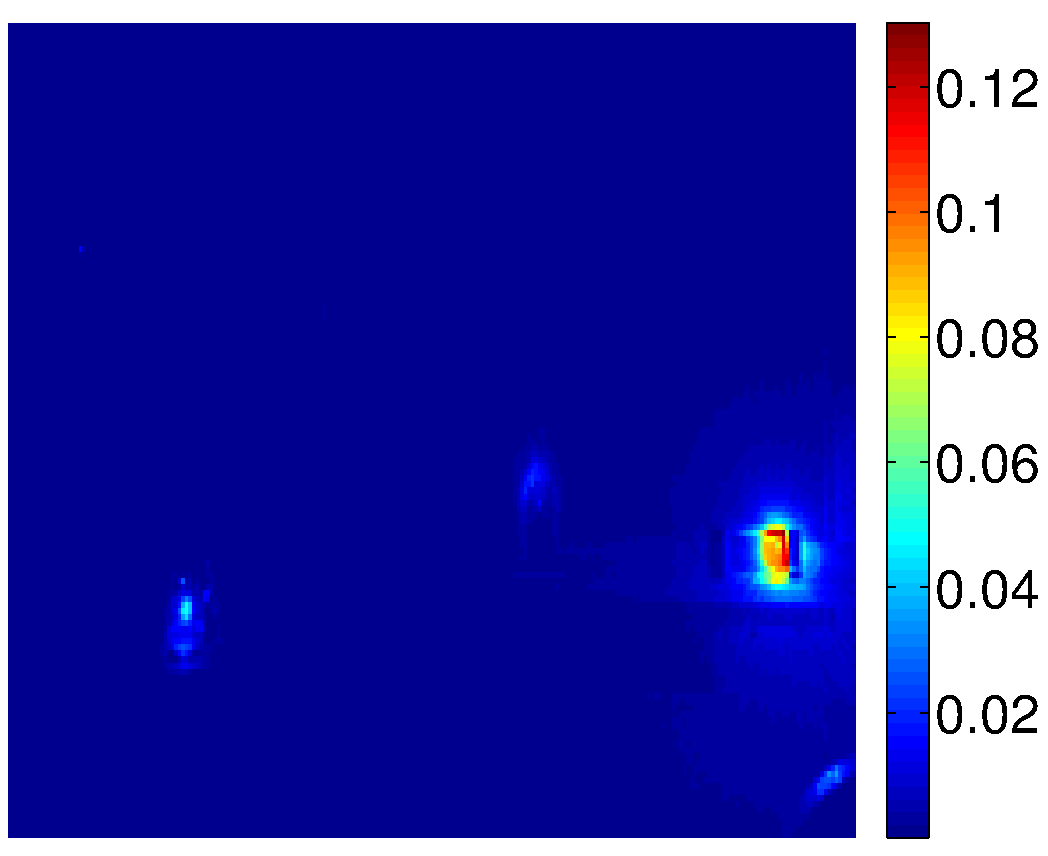
\includegraphics[width=0.45\textwidth]{figures/flashing1_left1_opt.pdf}\\[2ex]
      \hspace{-2ex}\textbf{Empirical CCA}\hspace{13ex}\textbf{ICCA - \iccap}\\
      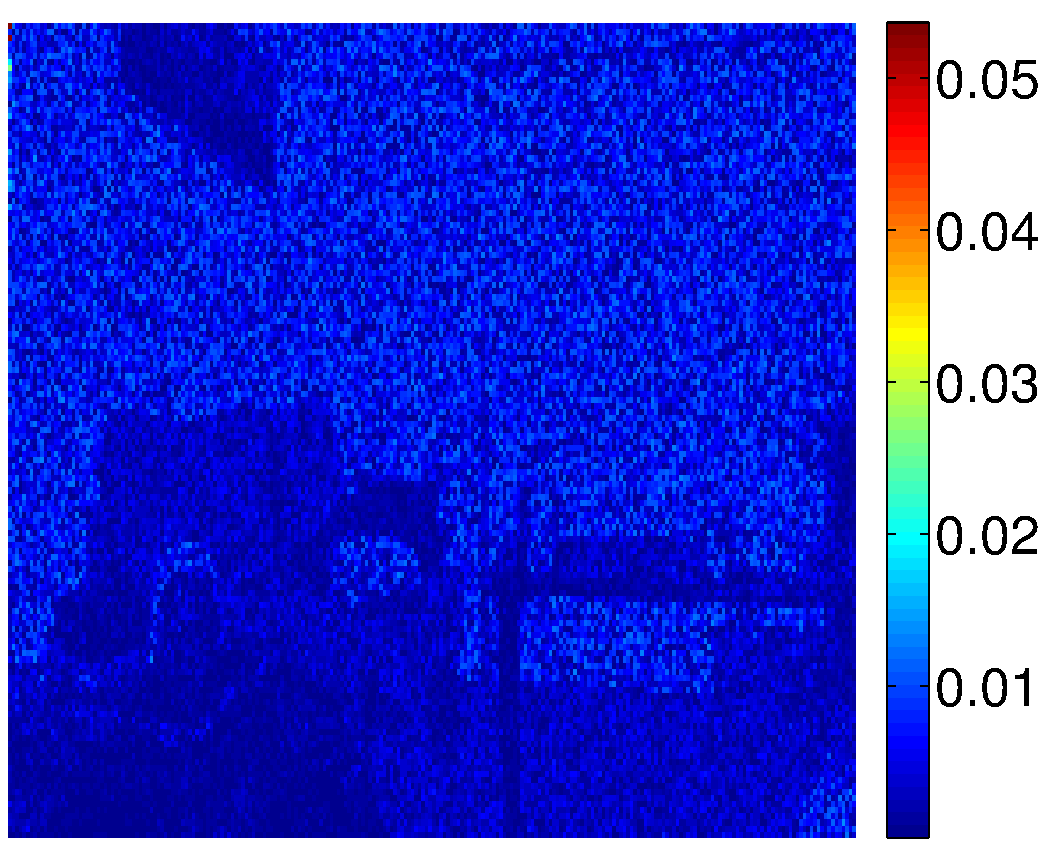
\includegraphics[width=0.45\textwidth]{figures/flashing1_left1_cca.pdf}\hspace{2ex}
      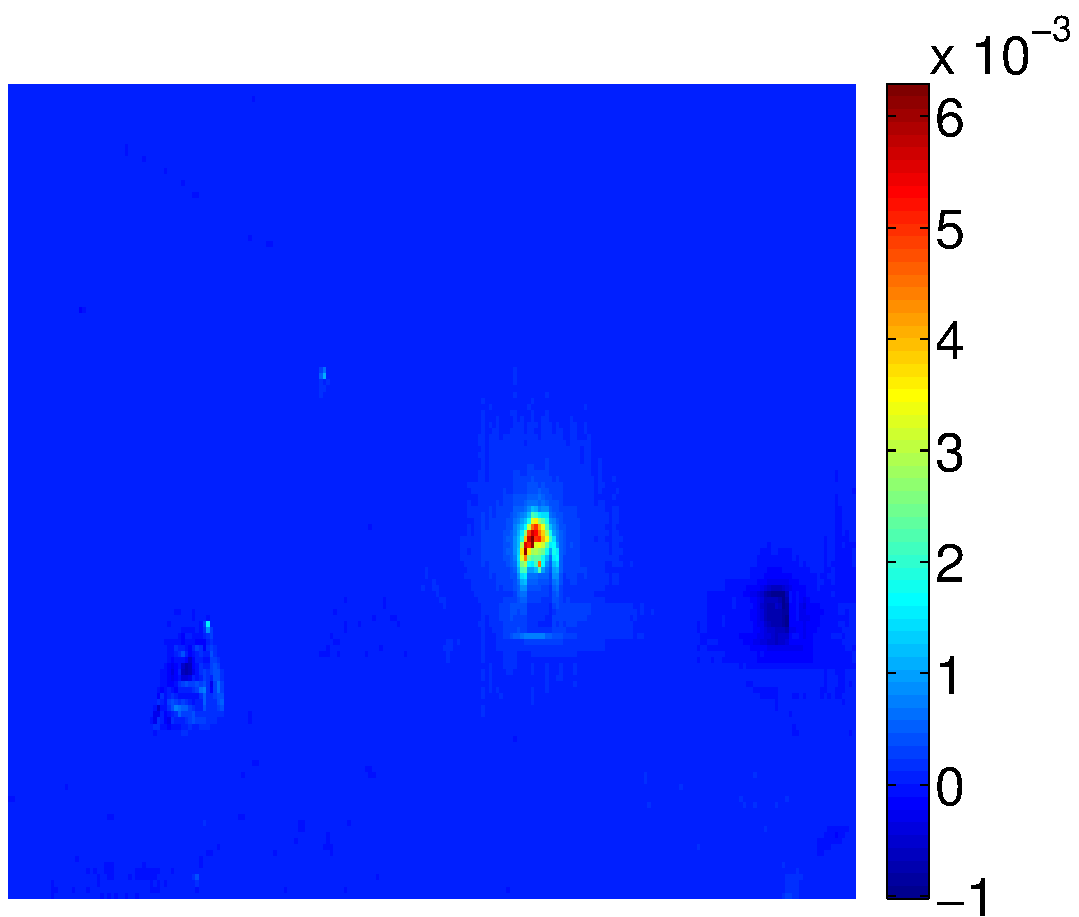
\includegraphics[width=0.45\textwidth]{figures/flashing1_left1_diff_icca.pdf}
    \end{center}
  \end{column}
\end{columns}
\end{frame}

%%%%%%%%%%%%%%%%%%%%%%%%%%%%%%%%%%%%%%%%%%%%%%%%%%%%%%%%%%%%%%%%%%%%%%%%%%%%%%
\begin{frame}{Correlation Analysis Wish List}
  \addtocounter{framenumber}{-1}

  \begin{center}
    \textbf{Correlation Algorithm Wish List}\\[1ex]
\fcolorbox{black}[HTML]{F1F1F1}{\parbox{0.8\textwidth}{%
    \begin{enumerate}
    \item \textcolor{texthigh}{\textbf{Reliable in the sample deficient regime} \checkmark}
      \begin{itemize}
      \item {\textcolor{texthigh}{meaningful correlations \checkmark}}
      \item \textcolor{texthigh}{meaningful canonical vectors \checkmark}
      \end{itemize}
    \item {\textcolor{texthigh}{\textbf{Statistical test for correlations} \checkmark}}
      \begin{itemize}
      \item {\textcolor{texthigh}{consistency analysis \checkmark}}
      \end{itemize}
    \item {\textcolor{texthigh}{\textbf{Robust} \checkmark}}
      \begin{itemize}
      \item {\textcolor{texthigh}{non-gaussian data \checkmark}}
      \item {\textcolor{texthigh}{missing data \checkmark}}
      \end{itemize}
    \item \textcolor{texthigh}{\textbf{Extends to more than 2 datasets} \checkmark}
    \end{enumerate}
}}
\end{center}

\end{frame}

%%%%%%%%%%%%%%%%%%%%%%%%%%%%%%%%%%%%%%%%%%%%%%%%%%%%%%%%%%%%%%%%%%%%%%%%%%%%%%
\begin{frame}{Analysis of $XY^H$ - Chpt. 6}

  \textbf{Recall key insight}
  \begin{itemize}
  \item $k = \Rank(\Ccca) = \Rank(\Rxy)$
  \end{itemize}

  \vspace{1ex}

  \begin{columns}[T!]
    \begin{column}{0.5\textwidth}
      \begin{center}
        \textbf{Simulation of $\sigma_i\left(XY^H\right)$ with noise}\\
        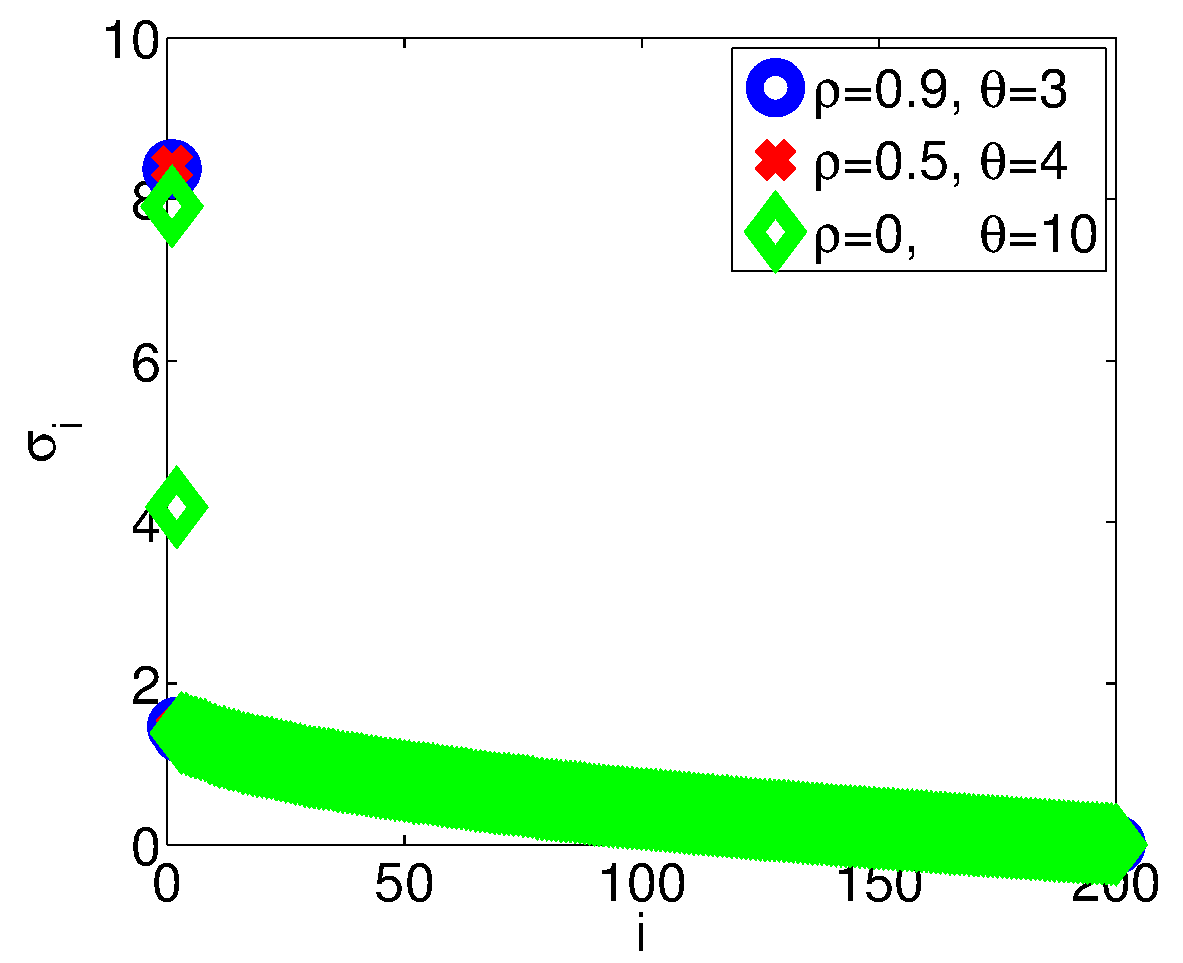
\includegraphics[width=0.8\textwidth]{figures/xy_motiv_pres.pdf}
      \end{center}
    \end{column}
    \begin{column}{0.5\textwidth}
      \textbf{Use SNR estimates}
      \begin{itemize}
      \item Pre-whiten the datasets 
      \item This is exactly CCA/ICCA!!
      \end{itemize}
    \end{column}
  \end{columns}

  \vspace{4ex}

  \textbf{Contributions}
  \begin{itemize}
  \item SVD of $XY^H$ is solution to regularized CCA as $\eta\to\infty$
  \item Almost sure limit of $\sigma_i\left(XY^H\right)$
  \end{itemize}

\end{frame}

\begin{frame}{SVD of Random Projections - Chpt. 7}



  \begin{center}
    \textbf{Signal-plus-noise Matrix}\\
    \fcolorbox{black}[HTML]{F1F1F1}{\parbox{0.5\textwidth}{
        \be
        \widetilde{X}_n= \sum_{i=1}^r\theta_i u_iv_i^T + X_n.
        \ee    
      }}
  \end{center}

\begin{columns}
  \begin{column}{0.4\textwidth}
  \begin{center}
  \textbf{Projections}\\
    \fcolorbox{black}[HTML]{F1F1F1}{\parbox{0.8\textwidth}{
        \be\ba
        &Y_n = P_n^H\widetilde{X}_n\\
        \ea\ee
      }}
  \end{center}
  \end{column}
  \begin{column}{0.6\textwidth}
    \vspace{2ex}
    \begin{itemize}
    \item $P_n=G_n\in\complex^{n\times m}$ with i.i.d. $\mathcal{CN}(0,1)$ entries
    \item $P_n=Q_n\in\complex^{n\times m}$ s.t. $Q_n^HQ_n = I_m$
    \end{itemize}
  \end{column}
\end{columns}

\vspace{2ex}

\begin{center}
  \textbf{Gaussian}\hspace{21ex}\textbf{Unitary}\phantom{hk}\\
 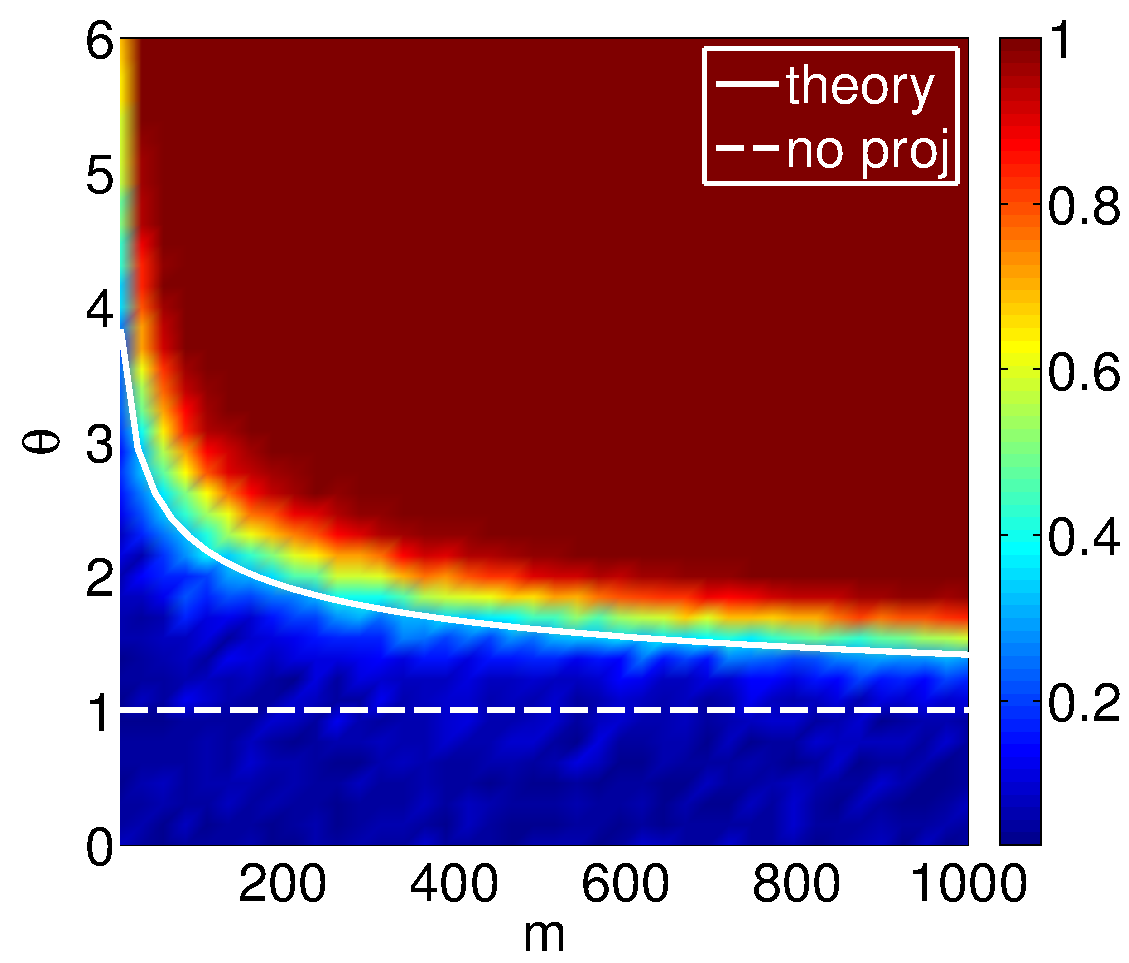
\includegraphics[width=0.35\textwidth]{figures/ks21.pdf}\hspace{2ex}
 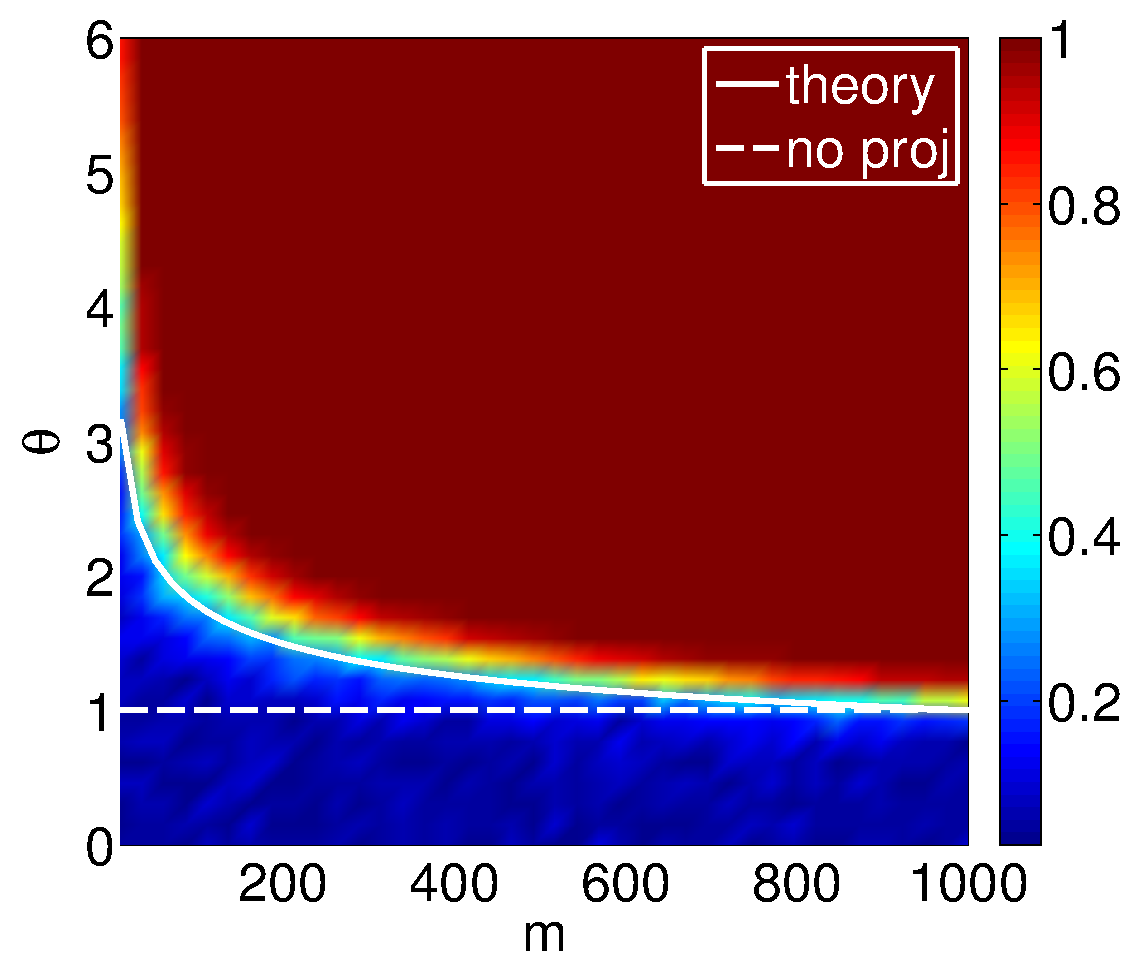
\includegraphics[width=0.35\textwidth]{figures/ks22.pdf}
\end{center}

\end{frame}



\begin{frame}{Content Based Image Retrieval}

  \begin{columns}
    \begin{column}{0.5\textwidth}

      \centering
      \textbf{Training Data}

      \vspace{-3ex}

      \begin{figure}
        \begin{center}
          \begin{tikzpicture}[
            font=\sffamily,
            every matrix/.style={ampersand replacement=\&,column sep=4ex},
            dataset/.style={draw,thick,fill=yellow!20,inner sep=.3cm},
            ellip/.style={draw=none,inner sep=.3cm},
            sink/.style={dataset,rounded corners,fill=black, text=white},
            app/.style={dataset,rounded corners,fill=blue!20},
            dots/.style={gray,scale=2},
            to/.style={->,>=stealth,shorten >=2pt,thick,font=\sffamily\footnotesize},
            every node/.style={align=center}]

            \matrix{       
              \node (data1) {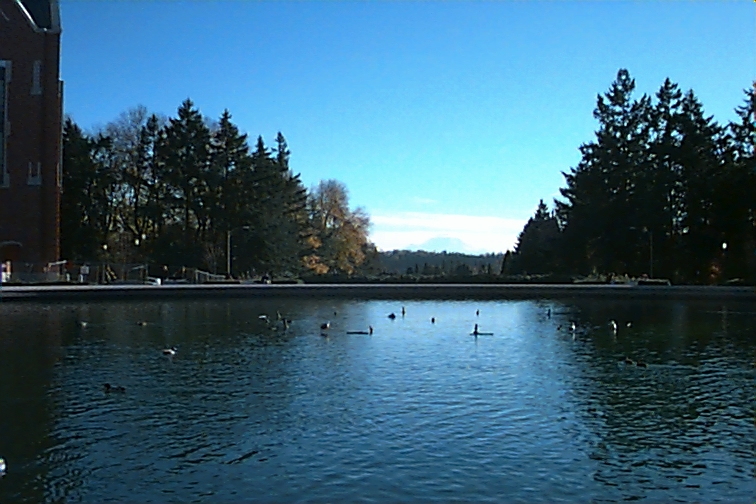
\includegraphics[width=0.5\textwidth]{figures/img_145.jpg}};
              \&\node[dataset] (cap1) {Caption 1};\\

              \node (data2) {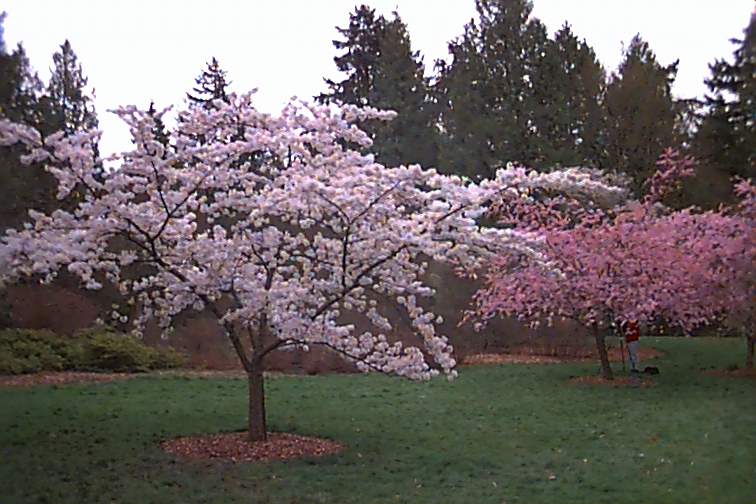
\includegraphics[width=0.5\textwidth]{figures/img_245.jpg}};
              \&\node[dataset] (cap2) {Caption 2};\\

              \node[ellip] (ell1) {$\vdots$};
              \&\node[ellip] (ell2) {$\vdots$};\\

              \node (data3) {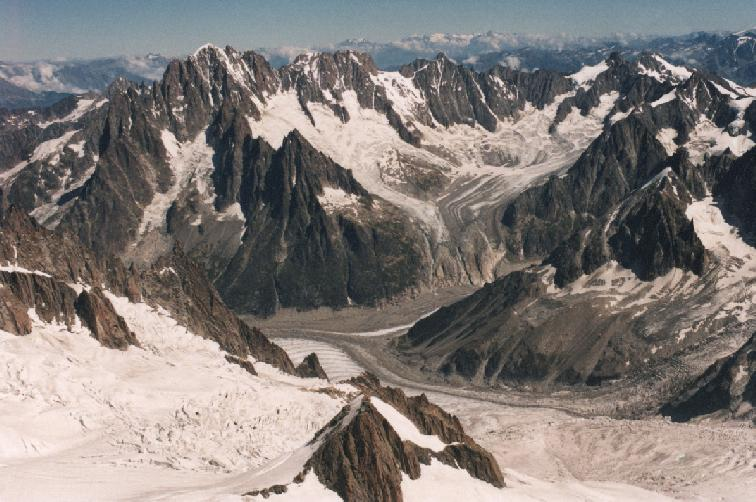
\includegraphics[width=0.5\textwidth]{figures/img_1049.jpg}};
              \&\node[dataset] (cap3) {Caption $n$};\\
            };

            \draw[to] (data1) -- (cap1) node[midway,left] {};
            \draw[to] (data2) -- (cap2) node[midway,left] {};
            \draw[to] (data3) -- (cap3) node[midway,left] {};

          \end{tikzpicture}
        \end{center}
      \end{figure}
    \end{column}
    \begin{column}{0.5\textwidth}
      \centering
      \textbf{Text Query}
      \begin{empheq}[box={\mybluebox[5pt][5pt][boxgrey]}]{equation*}
        \begin{aligned}
          & \text{snowy mountains}
        \end{aligned}
      \end{empheq}
      \Huge
      $$\Downarrow$$

      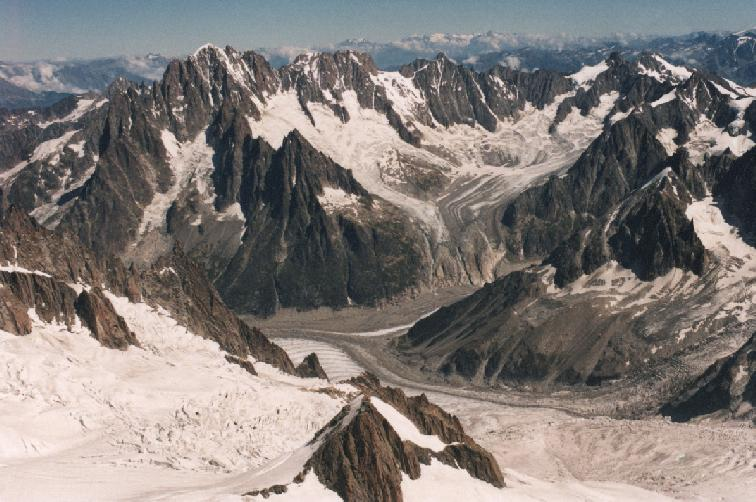
\includegraphics[width=0.5\textwidth]{figures/img_1049.jpg}
      

    \end{column}
  \end{columns}
\end{frame}

%%%%%%%%%%%%%%%%%
% Frame 2
%%%%%%%%%%%%%%%%%
\begin{frame}{Automatic Image Annotation}

  \begin{columns}
    \begin{column}{0.5\textwidth}

      \centering
      \textbf{Training Data}

      \vspace{-3ex}

      \begin{figure}
        \begin{center}
          \begin{tikzpicture}[
            font=\sffamily,
            every matrix/.style={ampersand replacement=\&,column sep=4ex},
            dataset/.style={draw,thick,fill=yellow!20,inner sep=.3cm},
            ellip/.style={draw=none,inner sep=.3cm},
            sink/.style={dataset,rounded corners,fill=black, text=white},
            app/.style={dataset,rounded corners,fill=blue!20},
            dots/.style={gray,scale=2},
            to/.style={->,>=stealth,shorten >=2pt,thick,font=\sffamily\footnotesize},
            every node/.style={align=center}]

            \matrix{       
              \node (data1) {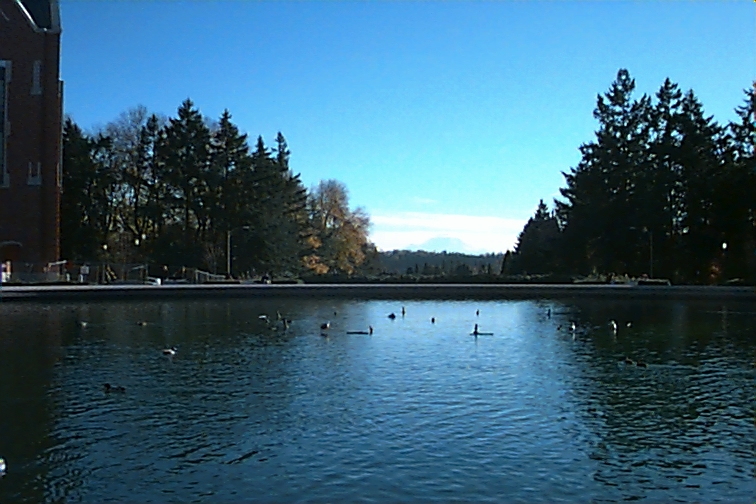
\includegraphics[width=0.5\textwidth]{figures/img_145.jpg}};
              \&\node[dataset] (cap1) {Caption 1};\\

              \node (data2) {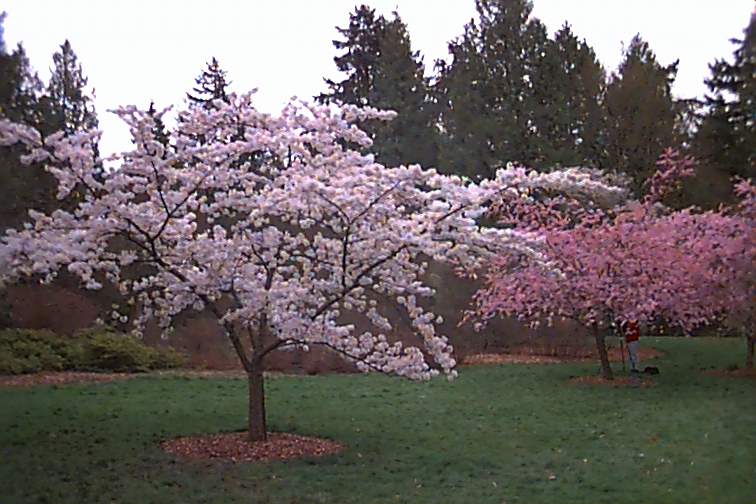
\includegraphics[width=0.5\textwidth]{figures/img_245.jpg}};
              \&\node[dataset] (cap2) {Caption 2};\\

              \node[ellip] (ell1) {$\vdots$};
              \&\node[ellip] (ell2) {$\vdots$};\\

              \node (data3) {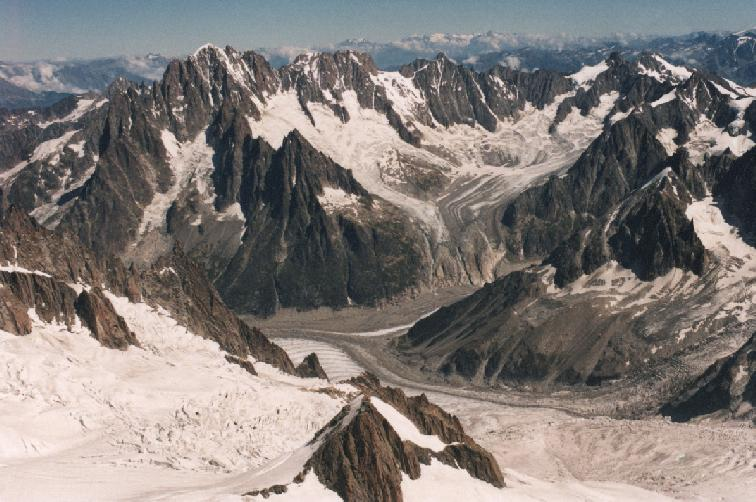
\includegraphics[width=0.5\textwidth]{figures/img_1049.jpg}};
              \&\node[dataset] (cap3) {Caption $n$};\\
            };

            \draw[to] (data1) -- (cap1) node[midway,left] {};
            \draw[to] (data2) -- (cap2) node[midway,left] {};
            \draw[to] (data3) -- (cap3) node[midway,left] {};

          \end{tikzpicture}
        \end{center}
      \end{figure}
    \end{column}
    \begin{column}{0.5\textwidth}
      \centering
      \textbf{Image Query}\\
      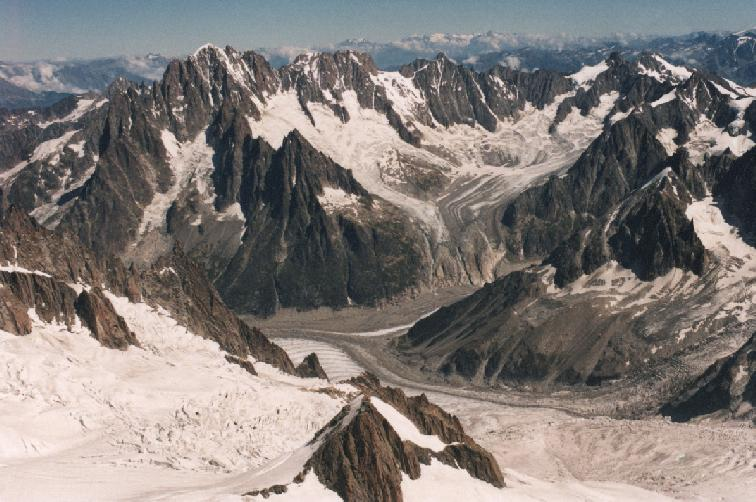
\includegraphics[width=0.5\textwidth]{figures/img_1049.jpg}
      {\Huge      $$\Downarrow$$}
      \begin{empheq}[box={\mybluebox[5pt][5pt][boxgrey]}]{equation*}
        \begin{aligned}
          & \text{snowy mountains}
        \end{aligned}
      \end{empheq}

    \end{column}
  \end{columns}
\end{frame}

\begin{frame}{Correlation Based Approaches}

  \textbf{Intuition}
  \begin{itemize}
  \item Image features are correlated to words
  \item CCA/ICCA seem like natural algorithms to identify correlations
  \end{itemize}

  \vspace{2ex}

  \textbf{Text Processing - \textit{\textcolor{textred}{tf}*\textcolor{texthigh}{idf}} feature vectors}
  \begin{itemize}
  \item \textcolor{textred}{term frequency} (\textit{tf}): frequent words are important
  \item \textcolor{texthigh}{inverse document frequency} (\textit{idf}): unique document words are important
  \item optional Porter stemming and stopword removal
  \end{itemize}

  \vspace{2ex}

  \textbf{Image Processing - Visual Words}
  \begin{enumerate}
  \item create SIFT features for all training images
  \item k-mean clustering of all SIFT features to ``visual words''
  \item assign each SIFT keypoint to closest visual word
  \item bag of words count the occurrences of visual word in each image
  \end{enumerate}

\end{frame}

\begin{frame}{Training Pipeline}

\begin{figure}
  \begin{center}
    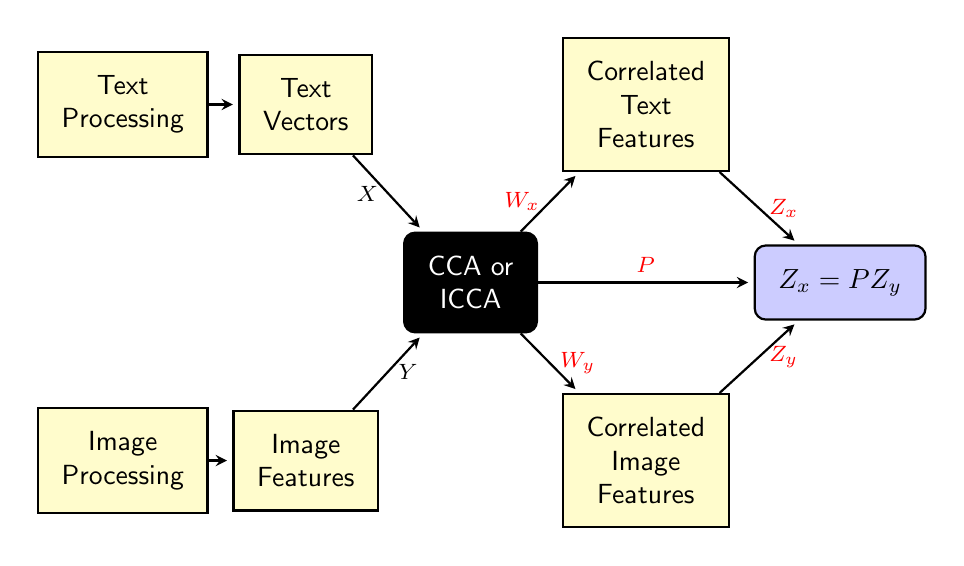
\begin{tikzpicture}[
      font=\sffamily,
      every matrix/.style={ampersand replacement=\&,column sep=2ex,row sep=5ex},
      dataset/.style={draw,thick,fill=yellow!20,inner sep=.3cm},
      sink/.style={dataset,rounded corners,fill=black, text=white},
      app/.style={dataset,rounded corners,fill=blue!20},
      dots/.style={gray,scale=2},
      to/.style={->,>=stealth,shorten >=2pt,thick,font=\sffamily\footnotesize},
      every node/.style={align=center}]

      \matrix{       
        \node[dataset] (textp) {Text \\ Processing};
        \& \node[dataset] (dataset1) {Text \\Vectors};
        \& ;
        \& \node[dataset] (dataset3) {Correlated \\Text \\Features};
        \&; \\

        ; 
        \& ;
        \& \node[sink] (blackbox) {CCA or\\ ICCA}; 
        \& ;
        \& \node[app] (application) {$Z_x=PZ_y$};\\

        \node[dataset] (imp) {Image \\Processing};
        \& \node[dataset] (dataset2) {Image \\Features};
        \& ;
        \& \node[dataset] (dataset4) {Correlated\\ Image\\ Features};
        \& ;\\
      };

      \draw[to] (textp) -- (dataset1)node[midway,left] {};
      \draw[to] (imp) -- (dataset2)node[midway,right] {};
      \draw[to] (dataset1) -- (blackbox)node[midway,left] {$X$};
      \draw[to] (dataset2) -- (blackbox)node[midway,right] {$Y$};
      \draw[to] (blackbox) -- (dataset3) node[midway,left] {\textcolor{red}{$W_x$}};
      \draw[to] (blackbox) -- (dataset4) node[midway,right] {\textcolor{red}{$W_y$}};
      \draw[to] (blackbox) -- (application) node[midway,above] {\textcolor{red}{$P$}};
      \draw[to] (dataset3) -- (application) node[midway,right] {\textcolor{red}{$Z_x$}};
      \draw[to] (dataset4) -- (application) node[midway,right] {\textcolor{red}{$Z_y$}};
    \end{tikzpicture}
  \end{center}
\end{figure}

\end{frame}

\begin{frame}{Automatic Caption Annotation Pipeline}

\begin{figure}
  \begin{center}
    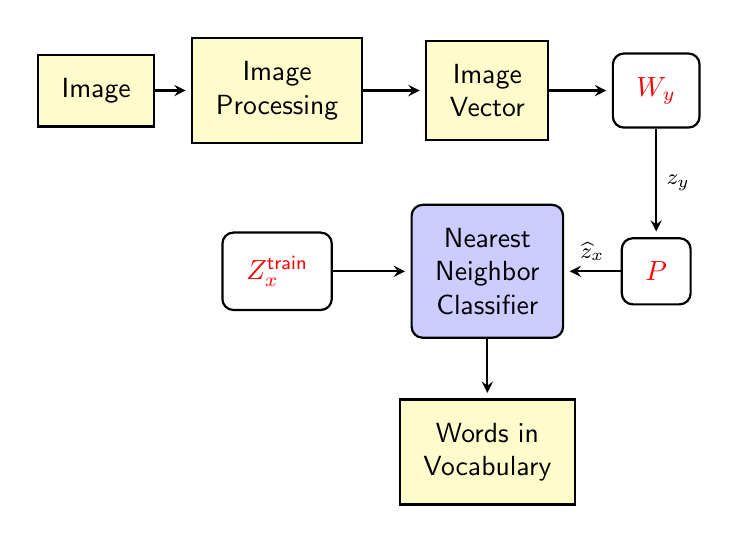
\begin{tikzpicture}[
      font=\sffamily,
      every matrix/.style={ampersand replacement=\&,column sep=3ex,row sep=5ex},
      dataset/.style={draw,thick,fill=yellow!20,inner sep=.3cm},
      sink/.style={dataset,rounded corners,fill=white, text=red},
      app/.style={dataset,rounded corners,fill=blue!20},
      dots/.style={gray,scale=2},
      to/.style={->,>=stealth,shorten >=2pt,thick,font=\sffamily\footnotesize},
      every node/.style={align=center}]


      \matrix{
        \node[dataset] (query) {Image};
        \& \node[dataset] (tp) {Image\\Processing};
        \& \node[dataset] (qv) {Image\\Vector};
        \&;\node[sink] (wx) {$W_y$};  \\

        ; 
        \& \node[sink] (zy) {$Z_x^{\text{train}}$}; 
        \& \node[app] (nn) {Nearest\\Neighbor\\Classifier};
        \& \node[sink] (P) {$P$}; \\

        ; 
        \& ;
        \& \node[dataset] (image) {Words in\\Vocabulary};
        \& \\
      };

      \draw[to] (query) -- (tp)node[midway,left] {};
      \draw[to] (tp) -- (qv)node[midway,right] {};
      \draw[to] (qv) -- (wx) node[midway,left] {};
      \draw[to] (wx) -- (P) node[midway,right] {$z_y$};
      \draw[to] (P) -- (nn) node[midway,above] {$\widehat{z}_x$};
      \draw[to] (zy) -- (nn) node[midway,right] {};
      \draw[to] (nn) -- (image) node[midway,right] {};


    \end{tikzpicture}
  \label{fig:training}
  \end{center}
\end{figure}

\end{frame}

\begin{frame}{Pascal Dataset}

  \textbf{Pascal Dataset}
  \begin{itemize}
  \item 1000 images each with 5 captions
  \item Vocabulary: 2393 words    
  \end{itemize}

\vspace{4ex}

\begin{figure}[T]
  \begin{minipage}{0.45\linewidth}
    \centering
    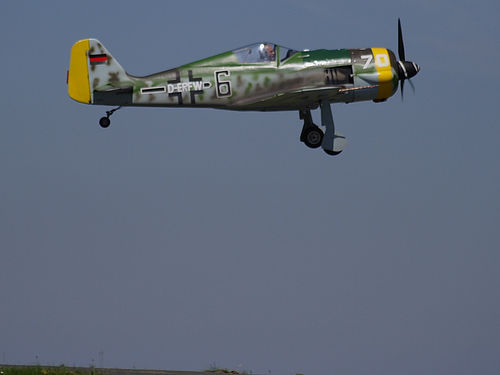
\includegraphics[width=.8\textwidth]{figures/img_3.jpg}
  \end{minipage}
  \begin{minipage}[t]{0.45\linewidth}
    \vspace{-10ex}
    \centering
    \footnotesize
    \begin{itemize}
    \item A D-ERFW-6 in flight.
    \item An army green plane flying in the sky.
    \item An old fighter plane flying with German military markings.
    \item A small green and yellow plane in the sky.
    \item A WWII fighter plane with its landing gear down.
    \end{itemize}
  \end{minipage}
\end{figure}



\end{frame}

%%%%%%%%%%%%%%%%%%%%%%%%%%%%%%%%%%%%%%%%%%%%%%%%%%%%%%%%%%%%%%%%%%%
\begin{frame}{Pascal Dataset - Image Retrieval}

\textbf{Text Query: } airplane

\vspace{3ex}

\begin{center}
  \textbf{CCA}\hspace{32ex}\textbf{ICCA}\\[0.5ex]
  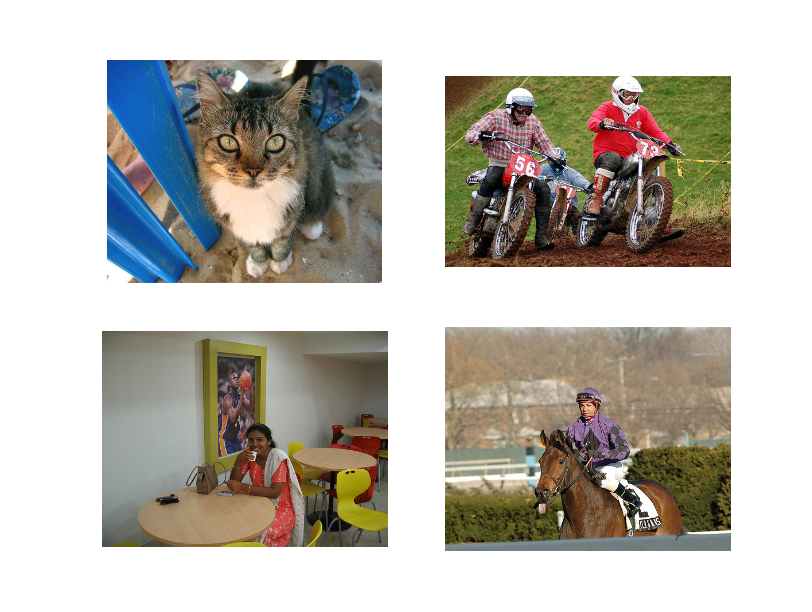
\includegraphics[width=0.45\textwidth]{figures/pascal_cca_ex.png}\hspace{2ex}
  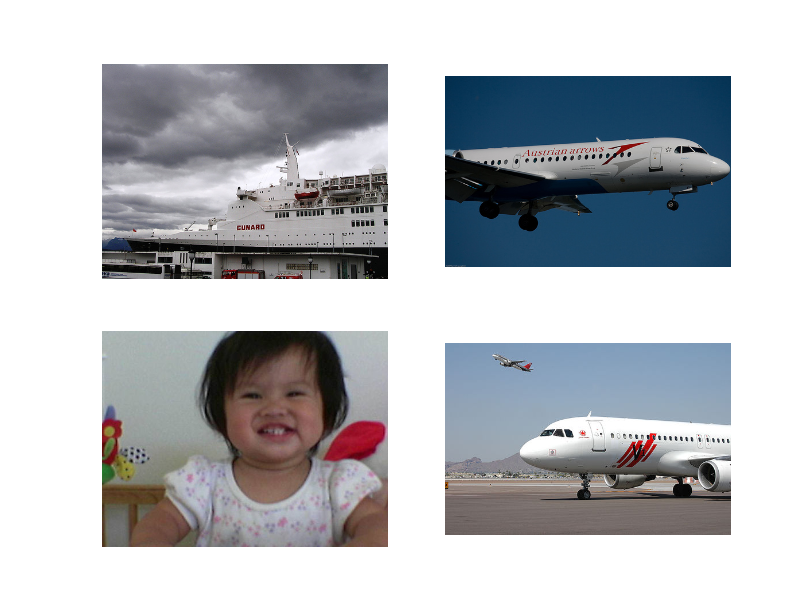
\includegraphics[width=0.45\textwidth]{figures/pascal_icca_ex.png}
\end{center}



\end{frame}


\begin{frame}{Pascal Dataset: Image Annotation}

\begin{columns}[T]
  \begin{column}{0.5\textwidth}
	\centering
    \textbf{Image Query}\\
	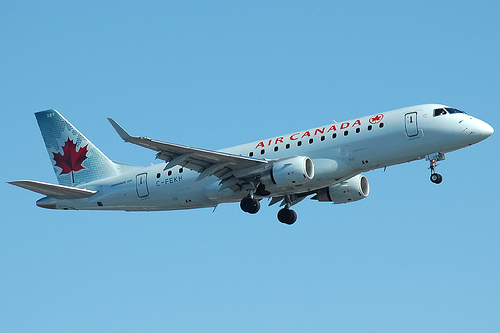
\includegraphics[width=0.8\textwidth]{figures/img_27.jpg}
  \end{column}
  \begin{column}{0.5\textwidth}
    \begin{minipage}[t]{0.4\textwidth}
      \small
      \begin{center}
        \textbf{CCA Annotation}
      \end{center}
      \begin{enumerate}
      \item hairless
      \item buddi
      \item swan
      \item leaf-less
      \item bnsf
      \item desert
      \item fluffi
      \item salad
      \item majest
      \item memorabilia
      \end{enumerate}
    \end{minipage}%
    \begin{minipage}[t]{0.1\textwidth}
    \end{minipage}
    \begin{minipage}[t]{0.4\textwidth}
      \small
      \begin{center}
        \textbf{ICCA Annotation}
      \end{center}
      \begin{enumerate}
      \item plane
      \item ship
      \item cruis
      \item fly
      \item blue
      \item jet
      \item airplan
      \item dock
      \item fighter
      \item through
      \end{enumerate}
    \end{minipage}
  \end{column}
\end{columns}
\end{frame}


%%%%%%%%%%%%%%%%%%%%%%%%%%%%%%%%%%%%%%%%%%%%%%%%%%%%%%%%%%%%%%%%%%%%%%%%%%%%%%
\begin{frame}{Correlation Analysis Wish List}
  \addtocounter{framenumber}{-1}

  \begin{center}
    \textbf{Correlation Algorithm Wish List}\\[1ex]
\fcolorbox{black}[HTML]{F1F1F1}{\parbox{0.8\textwidth}{%
    \begin{enumerate}
    \item \textcolor{texthigh}{\textbf{Reliable in the sample deficient regime} \checkmark}
      \begin{itemize}
      \item {\textcolor{texthigh}{meaningful correlations \checkmark}}
      \item \textcolor{texthigh}{meaningful canonical vectors \checkmark}
      \end{itemize}
    \item {\textcolor{texthigh}{\textbf{Statistical test for correlations} \checkmark}}
      \begin{itemize}
      \item {\textcolor{texthigh}{consistency analysis \checkmark}}
      \end{itemize}
    \item {\textcolor{texthigh}{\textbf{Robust} \checkmark}}
      \begin{itemize}
      \item {\textcolor{texthigh}{non-gaussian data \checkmark}}
      \item {\textcolor{texthigh}{missing data \checkmark}}
      \end{itemize}
    \item \textcolor{texthigh}{\textbf{Extends to more than 2 datasets} \checkmark}
    \end{enumerate}
}}
\end{center}

\end{frame}

\begin{frame}{Future Work}


\textbf{Kernel CCA}
\begin{itemize}
\item analysis for nonlinear low-rank signal-plus-noise model
\item analysis of choice of kernel
\item analysis of choice of regularization parameter
\end{itemize}

\vspace{2ex}

\textbf{MCCA}
\begin{itemize}
\item MAXVAR theorem for deterministic correlation when $n<\sum_i d_i$ 
\item null distribution for statistical test to estimate number of correlated signals
\item consistency analysis for estimate of number of correlated signals
\end{itemize}

\vspace{2ex}

\textbf{Image Annotation and Retrieval}
\begin{itemize}
\item clever feature engineering with NLP techniques 
\item extension to nonlinear algorithms
\end{itemize}



\end{frame}

\begin{frame}{Acknowledgments}

\textbf{Committee}
\begin{itemize}
\item Prof. Hero, Prof. Laura, Prof. Rada
\item Prof. Raj
\end{itemize}

\vspace{2ex}

\textbf{Colleagues}
\begin{itemize}
\item Nadakuditi group
\item GSC and SPeecs committees 
\item 3M ATG
\end{itemize}

\vspace{2ex}

\textbf{Friends}
\begin{itemize}
\item Hereford
\item University of Maryland
\item University of Michigan
\end{itemize}

\vspace{2ex}

\textbf{Family}

\end{frame}


\begin{frame}{\iccap Robustness to $\kxhat$ overestimation}

\begin{itemize}
\item $\kx=\ky=3$, $p=200$, $q=250$, $n=1000$,
$\Tx=\Ty=\diag(3,2,1)$, $\Pxy=\diag(0.9,0.5,0.3)$, $V_k=I_3$
\end{itemize}

\vspace{2ex}

\be
U_k= \left[\frac{1}{\sqrt{3}}\left[\begin{array}{c} 1\\ 1\\1\end{array}\right],
    \frac{1}{\sqrt{2}}\left[\begin{array}{c} 1\\
        0\\-1\end{array}\right],\frac{1}{\sqrt{6}}\left[\begin{array}{c} 1\\
        -2\\1\end{array}\right]\right]. 
\ee

\vspace{2ex}

\begin{center}
  \textbf{$w_x^{(1)}$}\hspace{22ex}\textbf{$w_x^{(2)}$}\hspace{22ex}\textbf{$w_x^{(3)}$}\\
    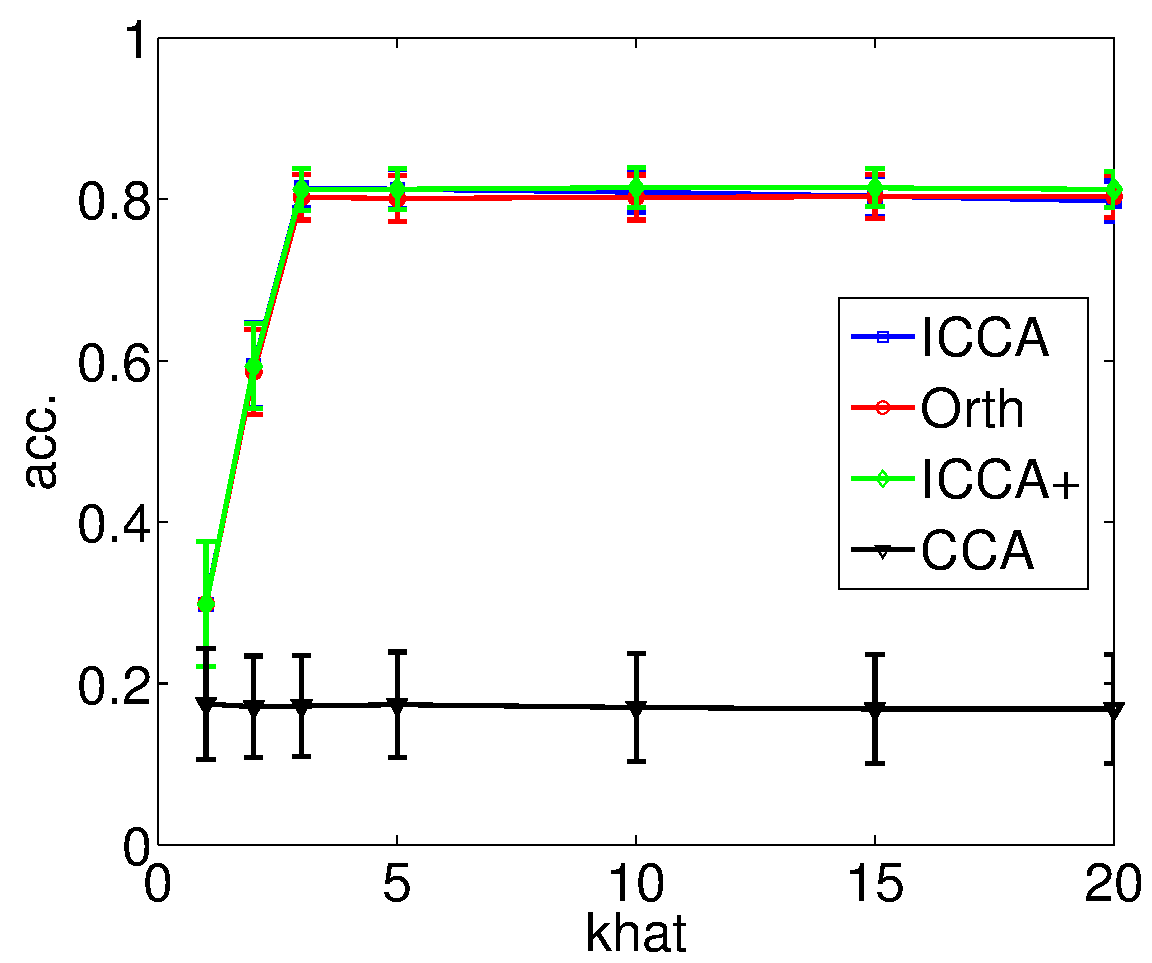
\includegraphics[width=0.3\textwidth]{figures/icca_vect_khat1_1.pdf}\hspace{2ex}
    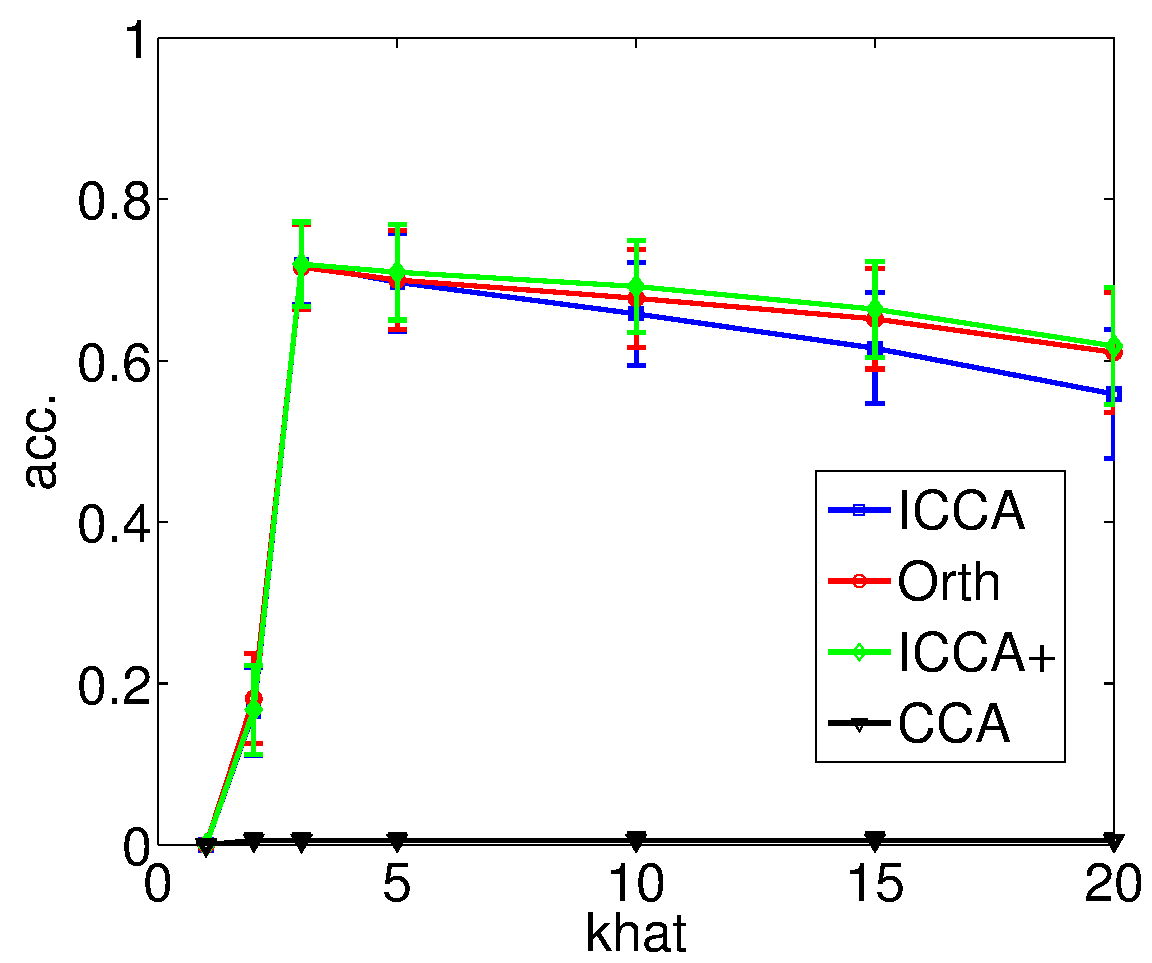
\includegraphics[width=0.3\textwidth]{figures/icca_vect_khat1_2.pdf}\hspace{2ex}
    \includegraphics[width=0.3\textwidth]{figures/icca_vect_khat1_3.pdf}
  \end{center}

\end{frame}

%%%%%%%%%%%%%%%%%%%%%%%%%%%%%%%%%%%%%%%%%%%%%
\begin{frame}{Limit of RCCA}

\begin{itemize}
\item AUC for signal vs. noise, $k=1$, $p=100$, $q=150$, $\rho=0.9$
\end{itemize}


  \setcounter{subfigure}{0}
  \begin{figure}
    \begin{center}
      \subfigure[$\eta=0.0001$]{       
        \includegraphics[width=0.35\textwidth]{figures/eta1_auc.pdf}
      }
      \subfigure[$\eta=0.01$]{       
        \includegraphics[width=0.35\textwidth]{figures/eta2_auc.pdf}
      }
      \subfigure[$\eta=10$]{       
        \includegraphics[width=0.35\textwidth]{figures/eta3_auc.pdf}
      }
      \subfigure[$\eta=1000$]{
        \includegraphics[width=0.35\textwidth]{figures/eta4_auc.pdf}
      }
    \end{center}
  \end{figure}

\end{frame}


\end{document}
